
\chapter{Multi-Sensor Profiling for Precision Soil-Moisture Monitoring}
\label{physics-aware-chap:pluto}

Controlling soil moisture is a crucial factor in optimizing watering and crop performance \cite{turkeltaub2016real}.
For instance, in our case study, Kiwifruit (\emph{Actinidia deliciosa}) -- in short Kiwi -- has high water demand \cite{judd1986water}, cultivated in countries such as New Zealand, Chile, and Italy.

Different types of watering systems may be adopted depending on the farming features and needs; typical solutions exploit drippers, sprinklers, hose reels, and flooding.
In orchards, where a stable watering system can be built, drip irrigation is widely used as it enables precise watering that, in turn, reduces water waste.

\paragraph{Challenges}
The risks of over-watering range from groundwater depletion to plant suffocation.
As to kiwi, farmers tend to over-water since it leads to larger fruits, but this reduces their dry mass and jeopardizes their maintenance after harvest.
Ideally, the moisture level should be known and optimal on the whole soil volume taken by the tree roots.
Such volume is subject to strong horizontal and vertical variability caused by many related factors, among them: (i) uneven root suction, (ii) limited watering-system coverage, and (iii) difference in the soil layers in terms of composition and exposure to atmospheric agents. %, (iv) punctual anomalies of the ground (e.g., hysteresis).

\Cref{pluto-fig:soilvolume} shows an example of an orchard watered through a single-pipeline dripper system.
Each cube shows the soil volume taken by the roots.
On the one hand, the limited distance between drippers ensures homogeneous moisture (i.e., the watered volume in blue) \textit{along the row} (i.e., multiple trees in the same line).
On the other hand, the effect of watering drops \textit{across the rows} (i.e., between two lines of trees), and a portion of the soil volume remains completely unwatered (i.e., the volume in orange).

When the watered volume is symmetric along the row, as in \Cref{pluto-fig:soilvolume}, a 2D grid (\Cref{pluto-fig:sensorgrid}-left) is sufficient to represent the entire soil volume. Conversely, when relevant moisture variations take place along the row too, a 3D grid (\Cref{pluto-fig:sensorgrid}-right) is more suitable. Such variations may be determined, for example, by too sparse drippers or by non-homogeneous suction of the roots.

\begin{figure}[t]
\centering
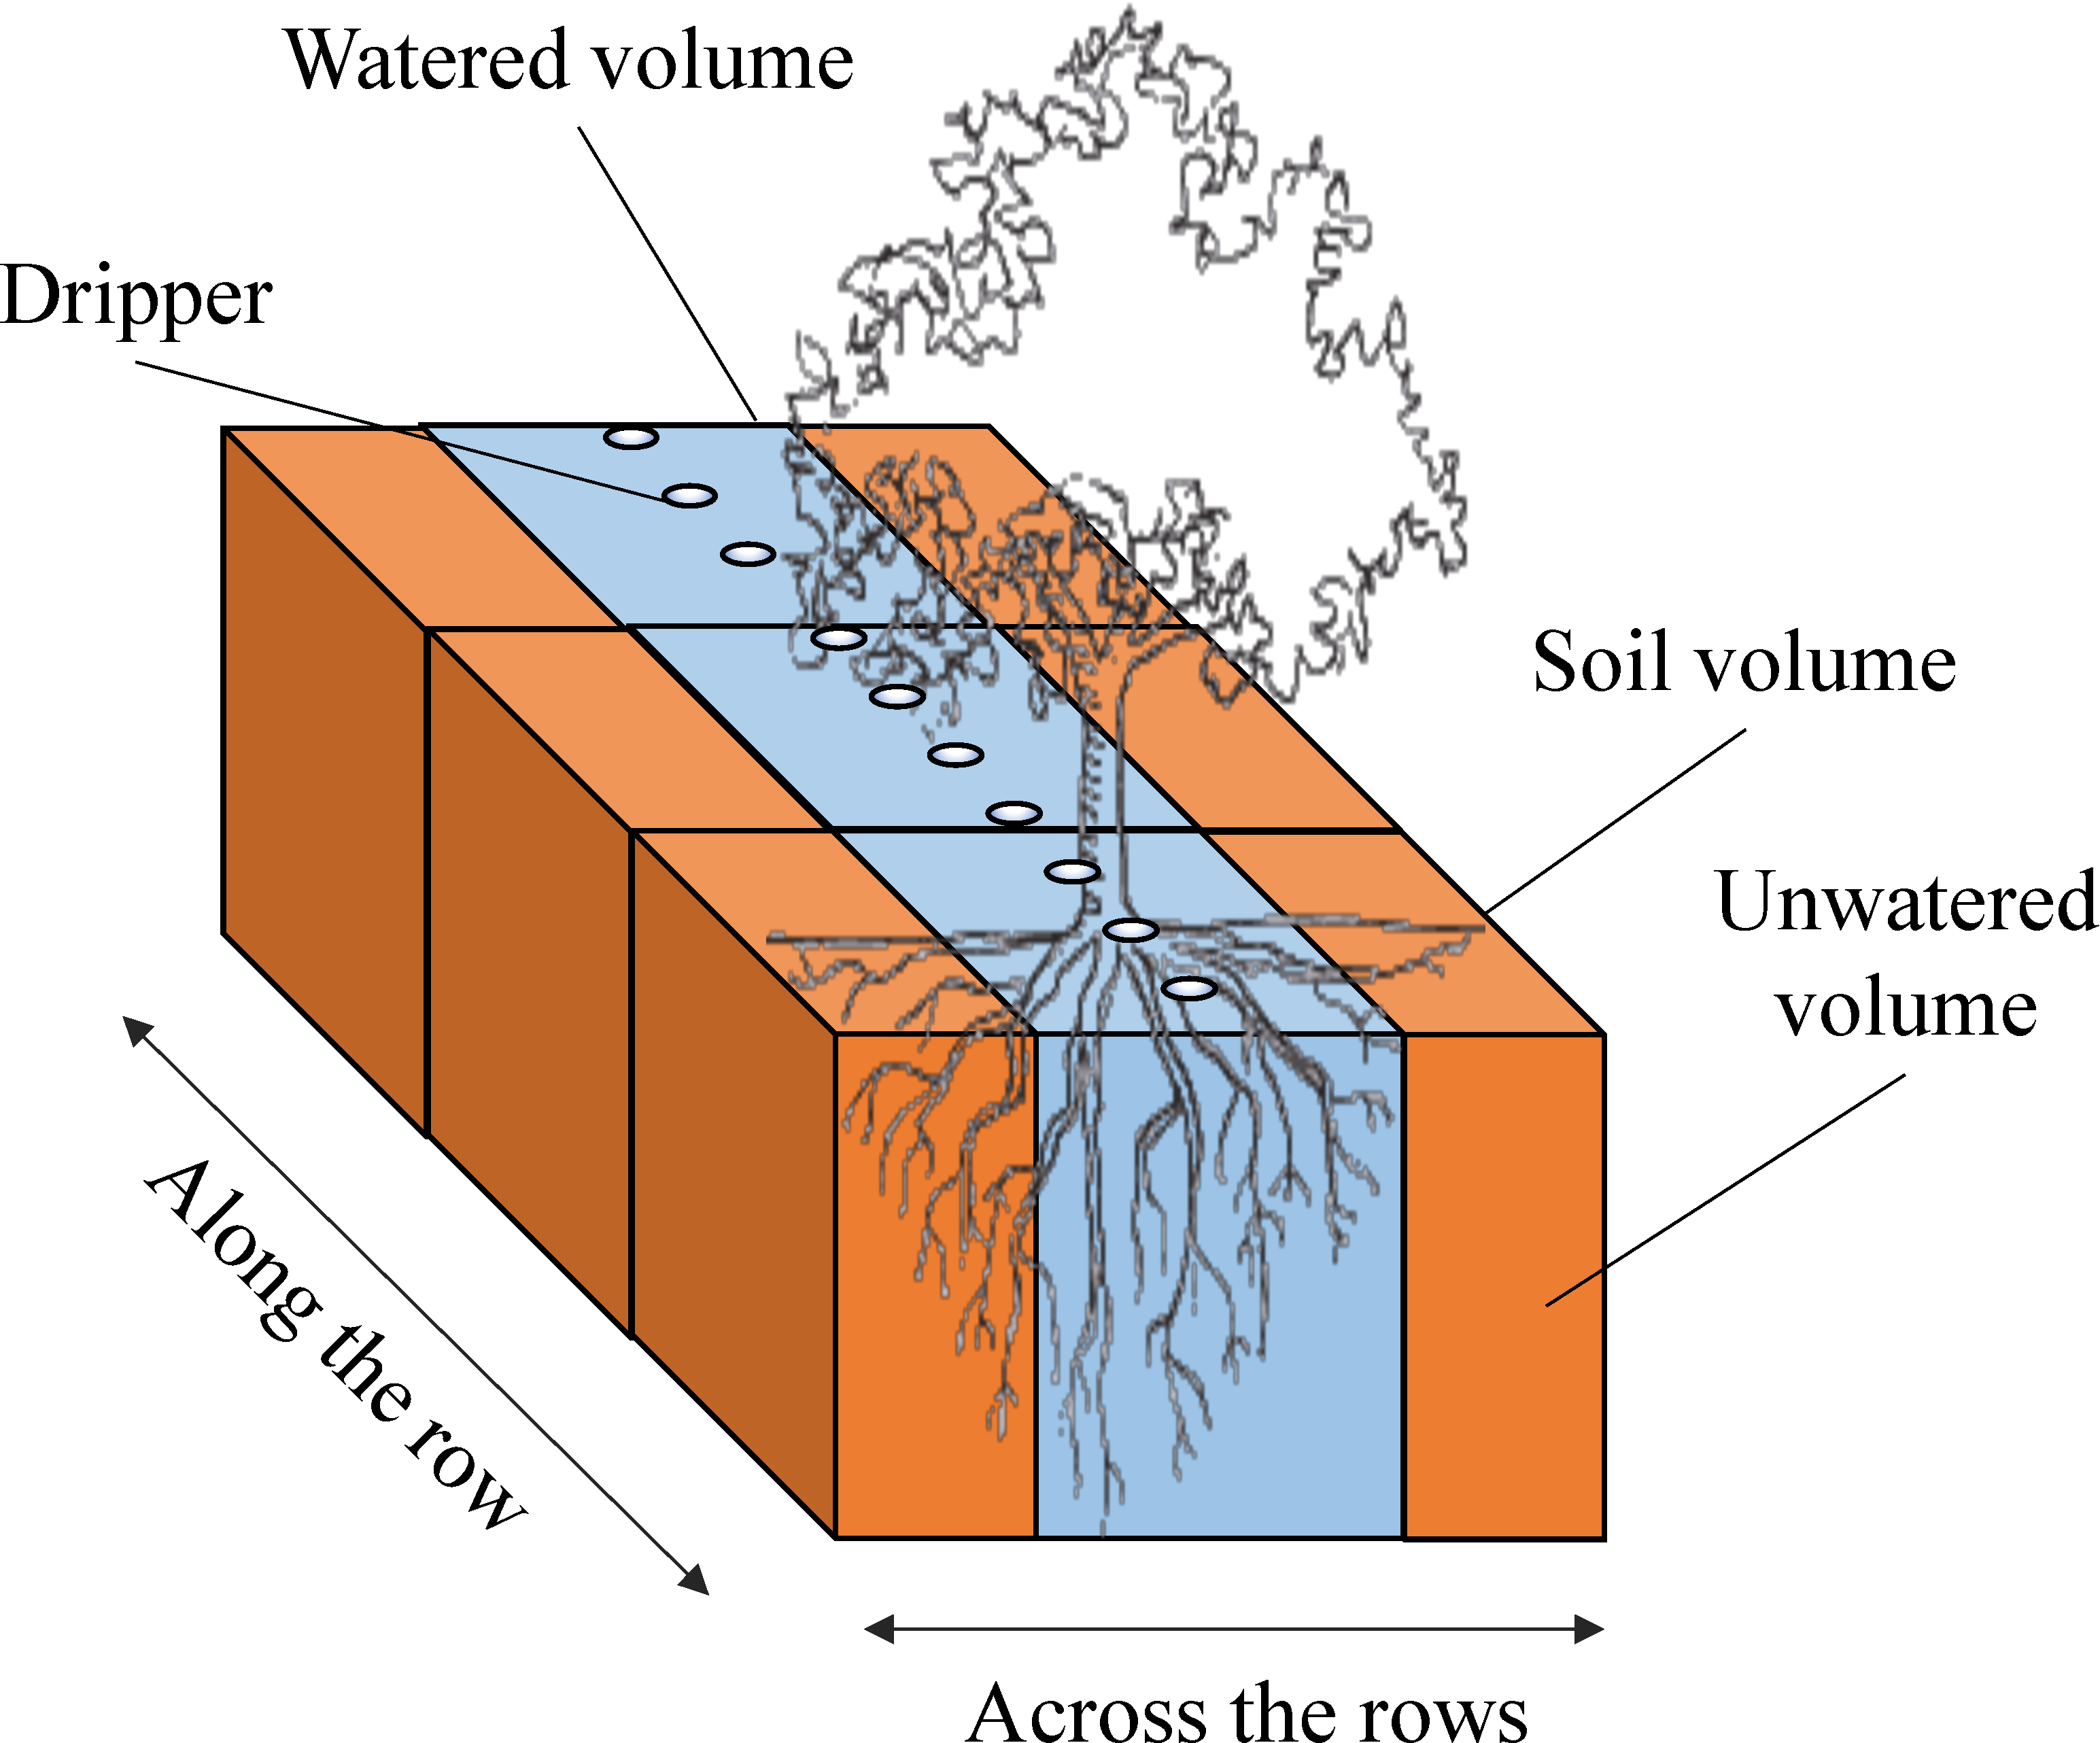
\includegraphics[scale=.14]{chapters/physics-aware/pluto/img/SoilVolume2.pdf}
\caption{Relevant elements in a orchard.}
\label{pluto-fig:soilvolume}
\end{figure}

\begin{figure}[t]
\centering
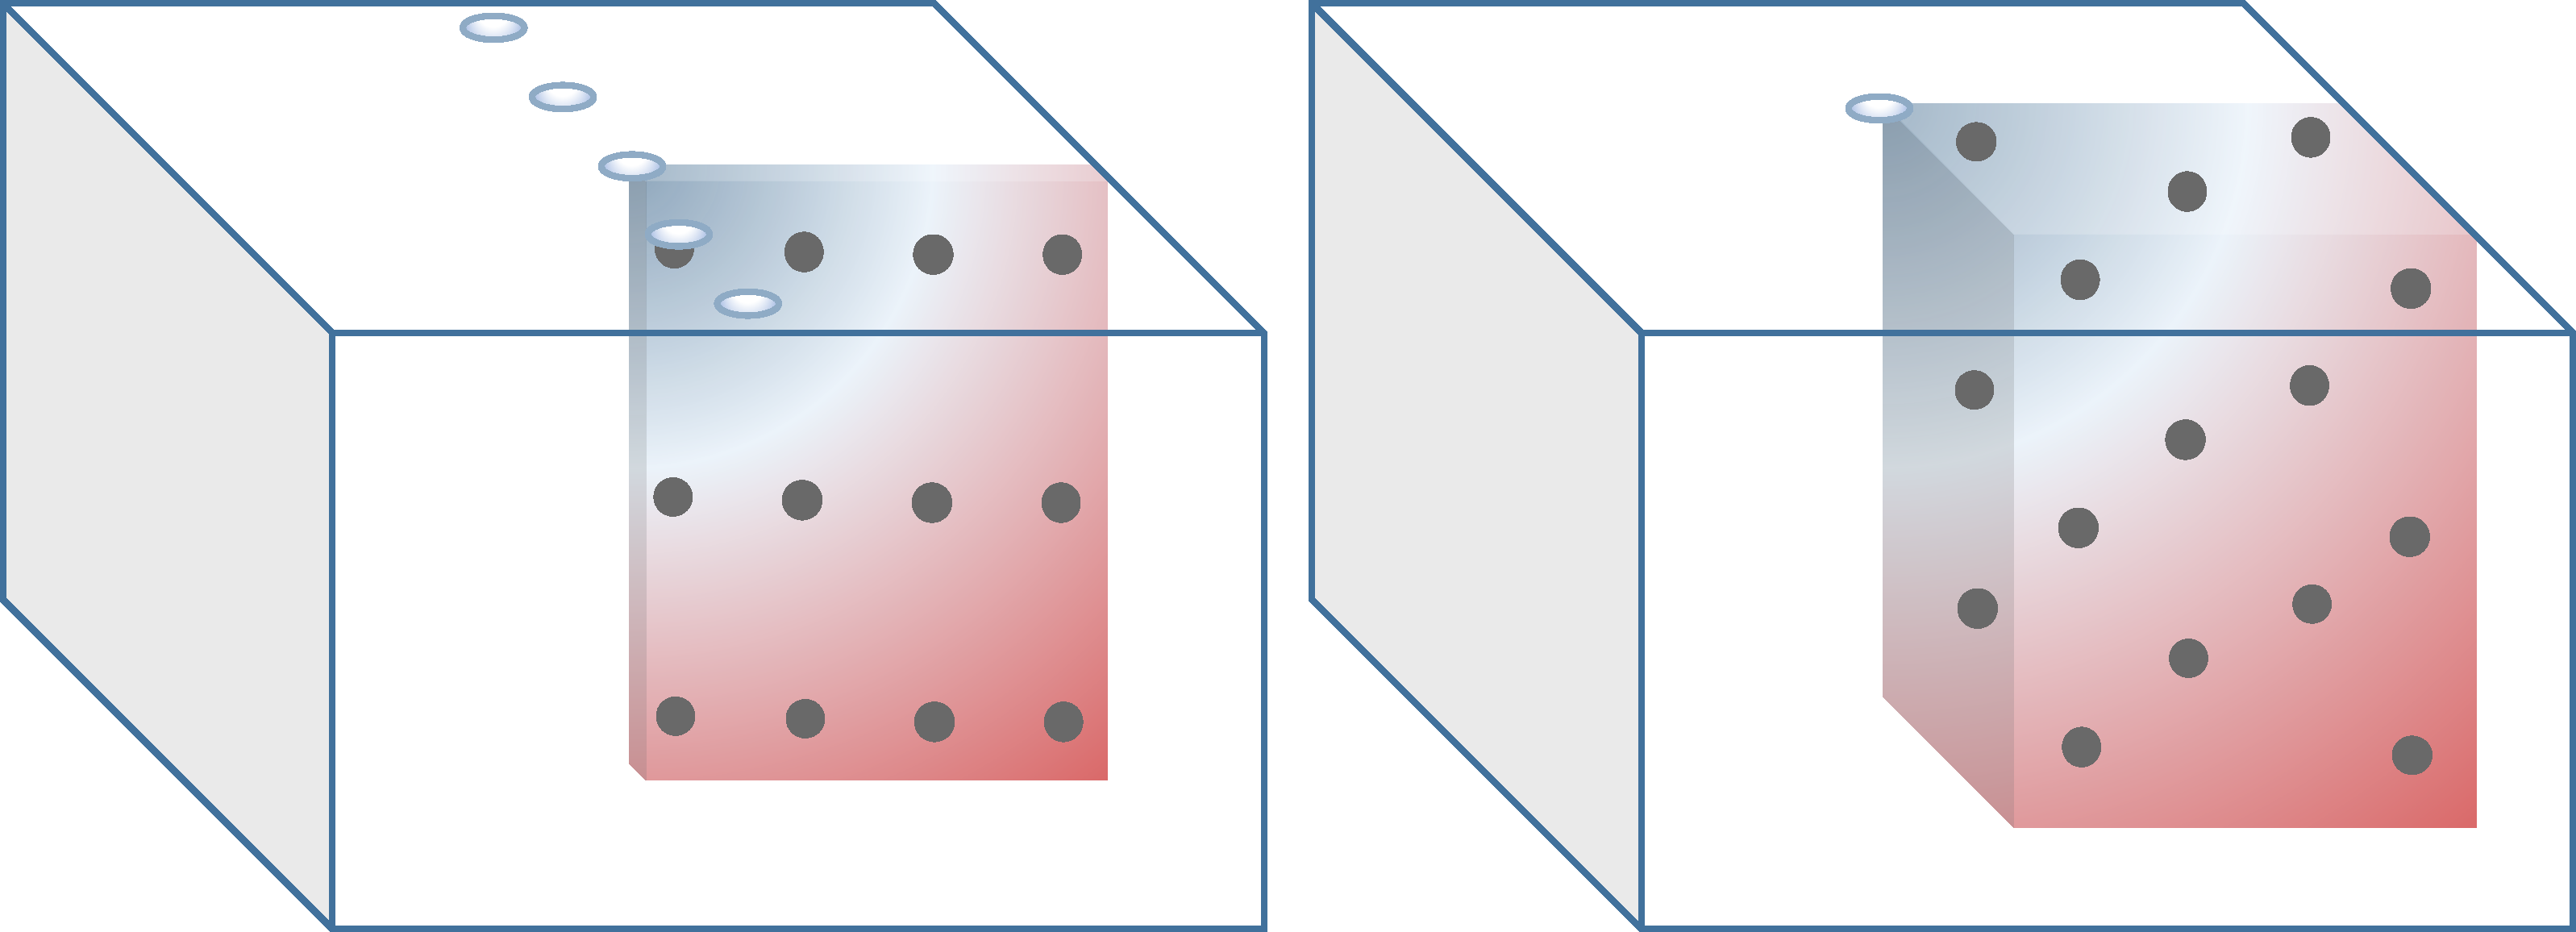
\includegraphics[scale=.21]{chapters/physics-aware/pluto/img/SensorGrid2.pdf}
\caption{Regular 2D (left) and 3D (right) sensor grids.}
\label{pluto-fig:sensorgrid}
\end{figure}

\paragraph{Contributions} The main application of our work is preserving an optimal moisture level without wasting water.
Our approach, named PLUTO\footnote{In Greek mythology, god of wealth. His name is linked to the prosperity of crops.}, focuses on the following contributions.
\begin{itemize}
    \item The concept of 2D/3D moisture profile (i.e., a fine-grained representation of moisture in a portion of soil) based on a grid of sensors. 
    The grain of the profile is in the order of magnitude of square/cubic centimeters.
    \item Two alternative solutions to estimate a fine-grained profile by adopting linear and non-linear approximations.
    In particular, non-linear approximation relies on a neural network that learns a model of soil moisture given the soil texture.
    \item An analysis of the trade-off between the accuracy, the number, and the position of sensors.
    \item Several original profile visualizations that enable visual exploitation of the profile.
\end{itemize}

To the best of our knowledge, PLUTO is the only approach aimed at creating a fine-grained multidimensional profile of soil moisture given a sensor grid.
In particular, previous approaches building a soil profile exploit sensors to calibrate a simulator (e.g., HYDRUS \cite{hydrus2008587}) and thus (i) require long time series of data from the field; (ii) bind the profile exploitation to an expensive and resource-consuming simulation; and (iii) require frequent updates.
For these reasons, such approaches typically carry out \textit{spot} researches to study soil moisture dynamics.
Conversely, our goal is to provide a cost-effective, operative solution that monitors soil moisture and whose reference application is \textit{long-term} watering optimization.

The remainder of this chapter is organized as follows. \Cref{pluto-sec:background} introduces the basics of soil moisture monitoring and surveys the previous related works in such an area.
\Cref{pluto-sec:MaterialsAndMethods} describes PLUTO in detail. Finally, \Cref{pluto-sec:ResultsAndDiscussion} reports the tests carried out on real data collected over two years, and \Cref{pluto-sec:conclusions} draws the conclusions.

We emphasize that our work is one of the outcomes of the Agro.Big.Data.Science project \cite{ABDS}.
The project, funded by Regione Emilia Romagna, aims at studying and implementing digital solutions to support smart and precision farming.

\section{Background and Related Works}
\label{pluto-sec:background}
The monitoring of soil moisture has been proven beneficial in many various applications.
For instance, \cite{Bordoni2018333} estimate the soil moisture on a test slope of Oltrepò Pavese (northern Italy) for the assessment of shallow landslides triggering.
Besides, agriculture has witnessed different analyses based on the adopted watering techniques.
Among them, the investigation of the water demand of a mature citrus orchard to optimize the water budget during rainy and dry seasons in southern China \cite{Tu2021}.
% In the field of flood irrigation, \cite{hamilton2020deepnew} collect soil moisture measurements and compare three contrasting soil management treatments, discovering how to improve efficiency.

In the following, we consider only papers related to precision farming, where it is important to have measurements as fine-grained as possible.
Specifically, we categorize them in \Cref{pluto-tbl:related} according different dimensions.
First, \Cref{orchard-ssec:sensors} analyzes the employed technology for data acquisition (i.e., Sensor Type and their Layout); then, \Cref{orchard-ssec:models} overviews the techniques leveraged to process the data for the ultimate goal (i.e., Model Type and Analysis Task).

\begin{table}[t]
    \centering
    % \footnotesize
    \caption{Classification and comparison of related works in the field of precision farming.}
    \begin{tabular}{llllll}
    \toprule
    Reference & Sensor Type & Layout & Model Type & Task \\ \midrule
    \cite{Pan2021}             & Volumetric      & multi (1D)    & Pb      & Studying  \\
    \cite{Li20152382}          & Volumetric      & multi (1D)    & Pb      & Studying  \\
    \cite{Egea2016197}         & Volumetric      & multi (2D)    & Pb      & Studying  \\
    \cite{Cordeiro2016139}     & Volumetric      & multi (2D)    & Pb      & Studying  \\
    \cite{Zapata-Sierra2021}   & Volumetric      & multi (3D)    & Pb      & Studying  \\
    \cite{chen2014spatial}     & Volumetric      & multi (1D)    & Pb      & Forecasting \\
    \cite{shein2019validation} & Potential       & multi (1D)    & Pb      & Forecasting \\
    \cite{arif2013estimation}  & Volumetric      & single (0D)   & ML       & Studying  \\
    \cite{Babaeian2021}        & UAS, Volumetric & multi (1D)    & ML       & Studying  \\
    \cite{Goldstein2018421}    & Volumetric      & multi (1D)    & ML       & Forecasting \\
    \cite{Jimenez20201327}     & Potential       & multi (1D)    & ML       & Forecasting \\
    \cite{Liang2021}           & Volumetric      & multi (3D)    & ML       & Forecasting \\
    \cite{Hinnell2010535}      & -               & -             & Pb, ML  & Profiling   \\
    PLUTO                      & Potential       & multi (2D/3D) & Pb, ML  & Profiling   \\ \bottomrule
    \end{tabular}
    \begin{tablenotes}
    \scriptsize
    \item Unmanned Aerial Systems (UAS), Process-based (Pb), Machine Learning (ML).
    \end{tablenotes}
    \label{pluto-tbl:related}
\end{table}

\subsection{Sensor Type and Layout}
\label{orchard-ssec:sensors}

The most common practice is to observe the change in soil moisture with the aid of sensors.
According to the displacement, sensors can be categorized as \textit{proximal} or \textit{remote}.
Proximal sensors are typically installed below the ground to monitor soil moisture in the plant root zone, offering precise measurements.
Conversely, remote sensors (e.g., Unmanned Aerial Systems) have been used for the discovery of global soil moisture patterns, due to their coarse spatial resolutions.
\cite{Babaeian2021} integrate both technologies to conduct analyses on global soil moisture patterns as well as near the plant.
Yet, commercial precision farming installations encompass only the use of proximal sensors, as including both sensor types is not worth the cost.
Furthermore, depending on the operating principle, proximal sensors measure either the \textit{volumetric water content} (i.e., the volume of liquid water per volume of soil) or the \textit{soil water potential} (i.e., the energy required by tree roots to extract water from soil particles).


Proximal sensors installations can be categorized into \textit{single-sensor} and \textit{multi-sensor} installations.
As the name suggests, the single sensor installation (0D) provides a punctual measurement of soil moisture.
Although this installation \cite{arif2013estimation} is cheap, it cannot monitor the soil moisture at different depths.
To do so, multi-sensor installations are devised (e.g., ground-based proximal sensors are organized so that a grid is formed).
According to the layout, we distinguish: mono-dimensional (1D), bi-dimensional (2D), and three-dimensional (3D) grids.
The most popular configuration is the mono-dimensional grid \cite{Karandish2016892, Goldstein2018421, Jimenez20201327, Pan2021, Li20152382}, where the sensors are vertically aligned at different depths.
Bi-dimensional \cite{Egea2016197, Cordeiro2016139} and three-dimensional \cite{Zapata-Sierra2021, Liang2021} grids are quite less used due to the higher required number of sensors.
Yet, they allow monitoring soil moisture changes not only at different depths but also along the other axes.
Bi-dimensional grids involve installations of multiple sensors per soil layer, forming thus a matrix that enables the understanding of patterns in an entire slice of soil.
While, three-dimensional grids can be seen as more bi-dimensional grids side by side, allowing the examination of more than one slice.
An exhaustive dissertation about sensors and data collection can be found in \cite{vitali2021crop}.

\subsection{Model Type and Analysis Task}
\label{orchard-ssec:models}

Raw sensory data are only the starting point for extracting richer representations of soil moisture.
We review the literature of approaches that
%, based on different techniques and with different goals,
have been proposed to create such representations.

First, we distinguish the approaches based on the employed modeling paradigm.
\begin{itemize}
    \item \emph{Machine Learning models} leverage artificial intelligence techniques to \textit{learn} hydrological dynamics from a large set of examples.
    \item \emph{Process-based models} (e.g., HYDRUS \cite{hydrus2008587}, CRITERIA \cite{Bittelli2011253}) are analytical models that \textit{encode} the physical laws determining the hydrological dynamics.
\end{itemize}
While we have a deep understanding of ML models, we provide a formal definition of a process-based model.

\begin{definition}[Process-based model \cite{Buck-Sorlin2013}]
    A process-based model is the mathematical (and normally computer-based) representation of one or several processes characterizing the functioning of well-delimited biological systems of fundamental or economic interest.
    Such models consist of a set of ordinary or partial differential equations that define the essence of each process, as well as their inputs and outputs.
\end{definition}

Such a modeling paradigm was heavily employed in the case of crop and soil modeling; for instance, processes in these cases might implement hydraulic fluxes or evapotranspiration.
Outputs of one process can serve as input to other processes, and so on and so forth, computing a series of time steps until the output of the final analysis is returned.
The overall computation is called \textit{simulation}, and such a paradigm was heavily employed in crop modeling.
For instance, in our case, the model simulates soil moisture dynamics across the whole irrigation season, in each soil unit, until the desired horizon is reached.

Besides, we distinguish the following Tasks.
\begin{itemize}
    \item \emph{Studying}, it estimates the soil dynamics over time with the aim of understanding the soil behavior under specific circumstances. A study is not bound to actual weather and soil moisture values, but rather tests different scenarios to understand the overall soil behavior.
    \item \emph{Forecasting}, starting from the current moisture values in a specific field, estimates its future values in order to let the user take appropriate decisions (e.g., watering).
    \item \emph{Profiling}, it estimates a fine-grained soil representation combining a coarse description of the moisture in the soil with statistical assumptions and the knowledge of soil characteristics.
\end{itemize}
Although the boundaries between these three goals are blurred, we can easily differentiate them considering that, while forecasting and study produce estimations of -- respectively -- \emph{future} and \emph{hypotethical} moisture values, profiling produces a more detailed estimate of \emph{present} values.

Process-based models have been for a long time the only choice to study hydrological dynamics, and thus are considered well-accepted and solid tools.
In this regard, several recent works exploit them with studying purposes: \cite{Pan2021} investigate the differences between two hole watering methods;  \cite{Li20152382} scrutinize the effects of soil water and salt dynamics on root water uptake; \cite{Egea2016197} analyze the suitability of the irrigation management of a hedgerow olive orchard in different soil types; \cite{Cordeiro2016139} determine the water table contribution in a cornfield; \cite{Zapata-Sierra2021} monitor the evolution of soil moisture in a pepper crop field.
As to works that focus on forecasting: \cite{chen2014spatial} predict the soil wetness status in several sites close to catchments of significant size (soil type and leaf area index were the key parameters affecting the model performance); \cite{shein2019validation} validate the efficiency of HYDRUS-1D for predicting soil moisture and temperature dynamics with hysteresis in clay loam soils.

ML models in the field of precision agriculture are relatively new in comparison to process-based models.
%Yet, they are pervasively leveraged and tested in each and every scientific area.
\cite{Karandish2016892} evaluate and compare the goodness of such models with process-based ones in several soil moisture simulations.
Results assess the efficacy of the former, which additionally benefit of some advantages, above all low resources consumption: no on-line heavy computation is required and the result is rapidly available.
As a matter of fact, several approaches apply ML with the aim of conducting studies: \cite{arif2013estimation} build a model to monitor soil moisture in paddy field with limited meteorological data; \cite{Babaeian2021} develop a ML model that analyzes surface, near-surface, and root zone soil moisture by exploiting the fusion of remote and proximal sensors.
As to forecasting: \cite{Liang2021} quantify the water droplet infiltration in a sprinkler irrigation system to improve and facilitate the watering management, \cite{Jimenez20201327} and \cite{Goldstein2018421} directly predict the watering volumes recommended by the agronomist.

Finally, there are approaches that leverage process-based models in synergy with ML.
For instance, \cite{Hinnell2010535} exploit HYDRUS as a process-based model to provide fine-grained samples and Artificial Neural Networks as a ML model to extract subsurface wetting patterns. With respect to PLUTO, \cite{Hinnell2010535} (i) produce a statistical representation of the patterns that is based on a \textit{single} dripper and assume a \textit{uniform} characterization of the soil, (ii) derive the wetting patterns from generic soil parameters and not from actual sensor values.
% However, they do not utilized any real soil moisture measurements to calibrate the numerical model.
% Indeed, it is well-known that realistic simulations with process-based models require real soil moisture measurements to correctly model all the soil phenomena (e.g., water tables, hysteresis).

% \Cref{pluto-tbl:related} summarizes the related works described so far and compares their features against PLUTO. 
% To the best of our knowledge, PLUTO is the only one that builds a fine-grained 2D/3D moisture profile based on a coarser sensors grid, through linear and non-linear techniques.



\section{PLUTO}
\label{pluto-sec:MaterialsAndMethods}
\begin{figure}[t]
\centering
\begin{subfigure}[t]{.3\textwidth}
\centering

\includegraphics[scale=.15]{chapters/physics-aware/pluto/img/soil-moisture-continuous.pdf}
\caption{Actual soil moisture.}
\label{pluto-fig:moisture-cont}
\end{subfigure}~
\begin{subfigure}[t]{.3\textwidth}
\centering
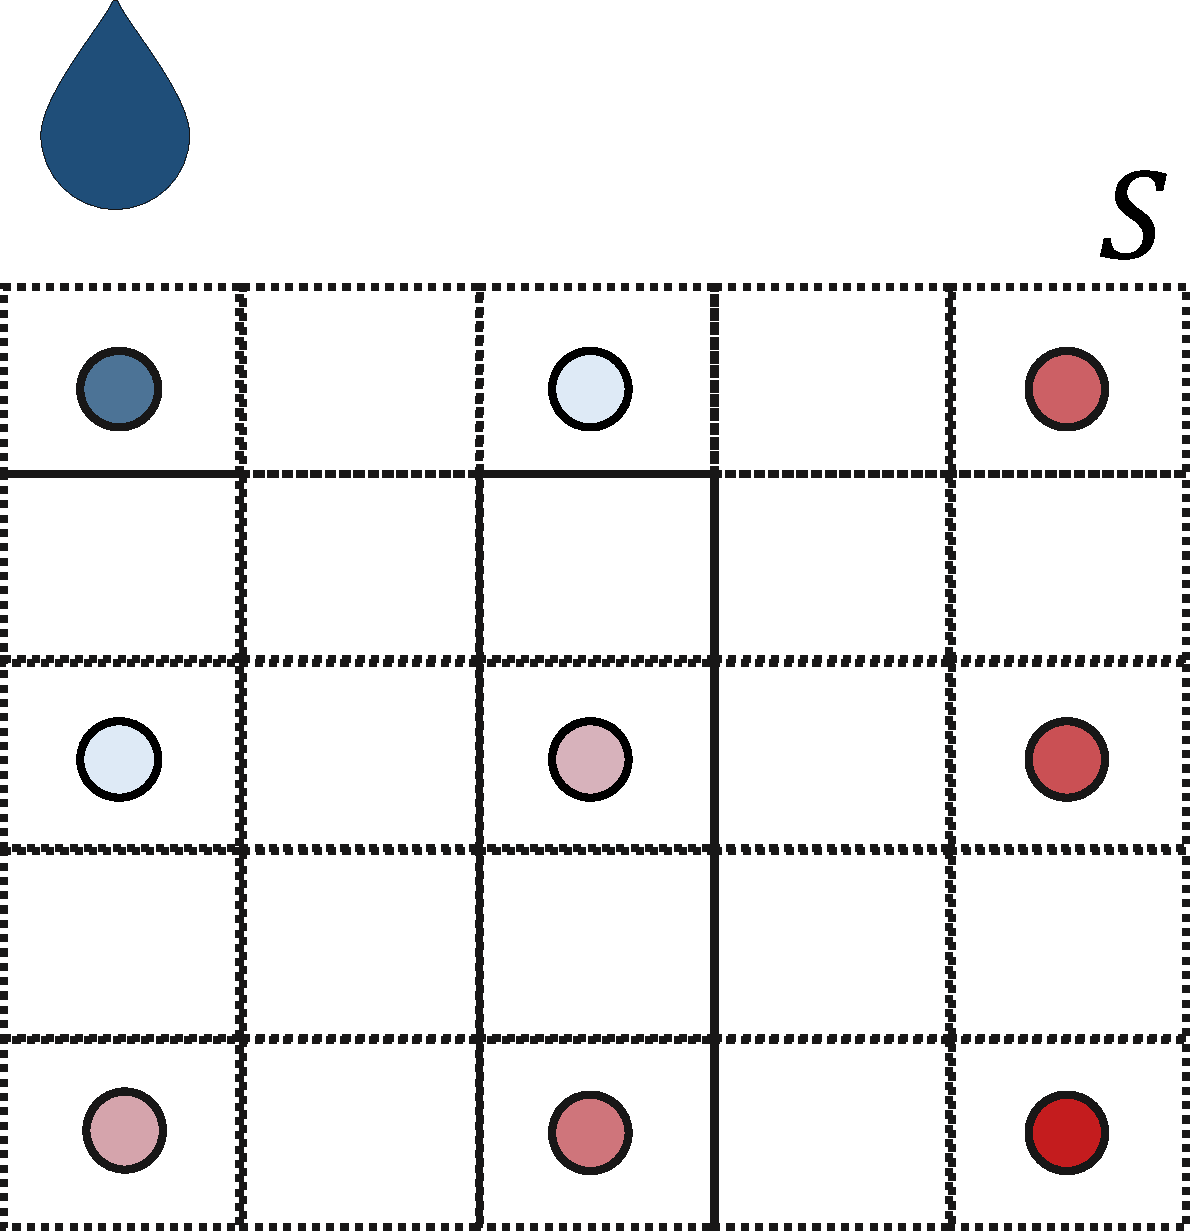
\includegraphics[scale=.15]{chapters/physics-aware/pluto/img/soil-moisture-sample.pdf}
\caption{Raw sensor grid}
\label{pluto-fig:moisture-sens}
\end{subfigure}
~
\begin{subfigure}[t]{.3\textwidth}
\centering
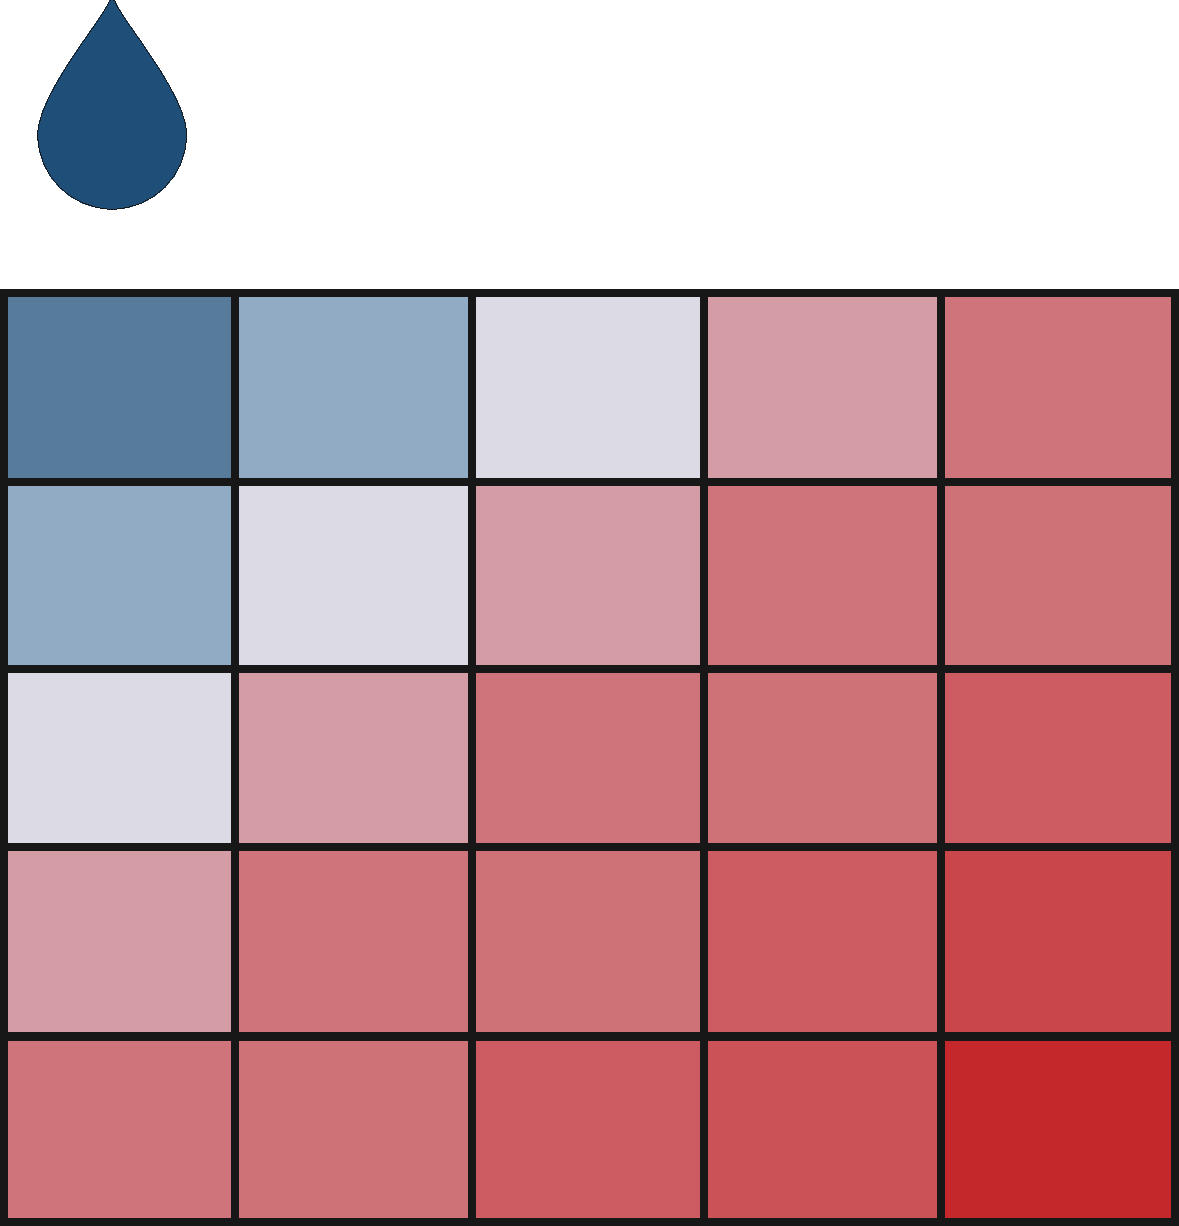
\includegraphics[scale=.15]{chapters/physics-aware/pluto/img/soil-moisture-profile.pdf}
\caption{Soil profile}
\label{pluto-fig:moisture-profile}
\end{subfigure}
\caption{Snapshot of soil moisture in a soil slice; the water drop represents a dripper.}
\label{pluto-fig:moisture}
\end{figure}

Our goal is to create a moisture profile that represents the whole soil volume.
\begin{definition}[Soil volume]
Given a tree, its \emph{soil volume} is a parallelepiped of soil that contains most of the tree roots. The soil volume is centered in the tree position.
\end{definition}

\begin{definition}[Sensor grid]
A \emph{sensor grid} $S = \{s^1, ..., s^{|S|}\}$ is an $n$-dimensional layout of $|S|$ sensors installed in a soil volume.
Each \emph{sensor} $s^i$ is defined by a three-dimensional displacement $(s^i.x_1, s^i.x_2,s^i.x_3)$ with respect to the center of the soil volume, and by a soil moisture value $s^i.v$. 
\end{definition}


Depending on $n$, the grid resembles a line ($n=1$), a rectangle ($n=2$) or a parallelepiped ($n=3$). The monitored value depends on the sensor technology; typically sensors measure volumetric water content or the soil potential. \Cref{pluto-fig:installation} shows one of the Agro.Big.Data.Science project installations \cite{ABDS} located in Faenza (Emilia Romagna, Italy).
This orchard is watered through a single pipeline of drippers (distance between drippers 40cm) and soil moisture is monitored through a 2D sensor grid of 12 gypsum block sensors.

\begin{figure}[t]
    \centering
    \begin{subfigure}[t]{.5\textwidth}
    \centering
    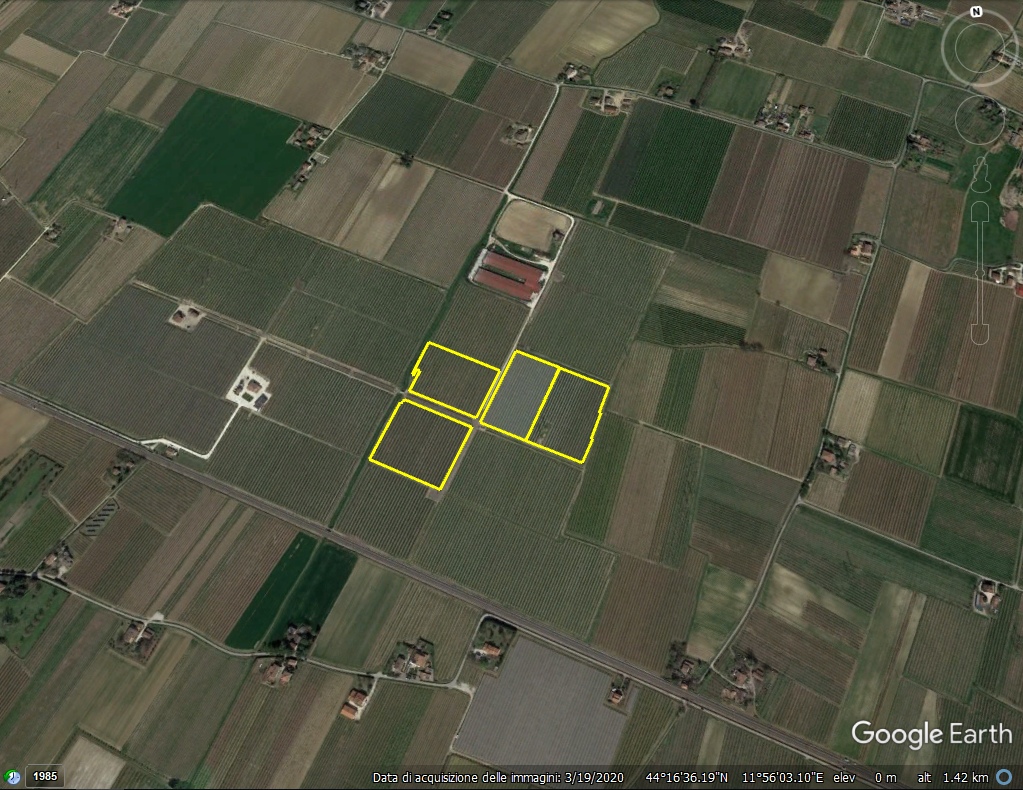
\includegraphics[scale=.145]{chapters/physics-aware/pluto/img/sensors-satellite.png}
    \end{subfigure}~
    \begin{subfigure}[t]{.5\textwidth}
    \centering
    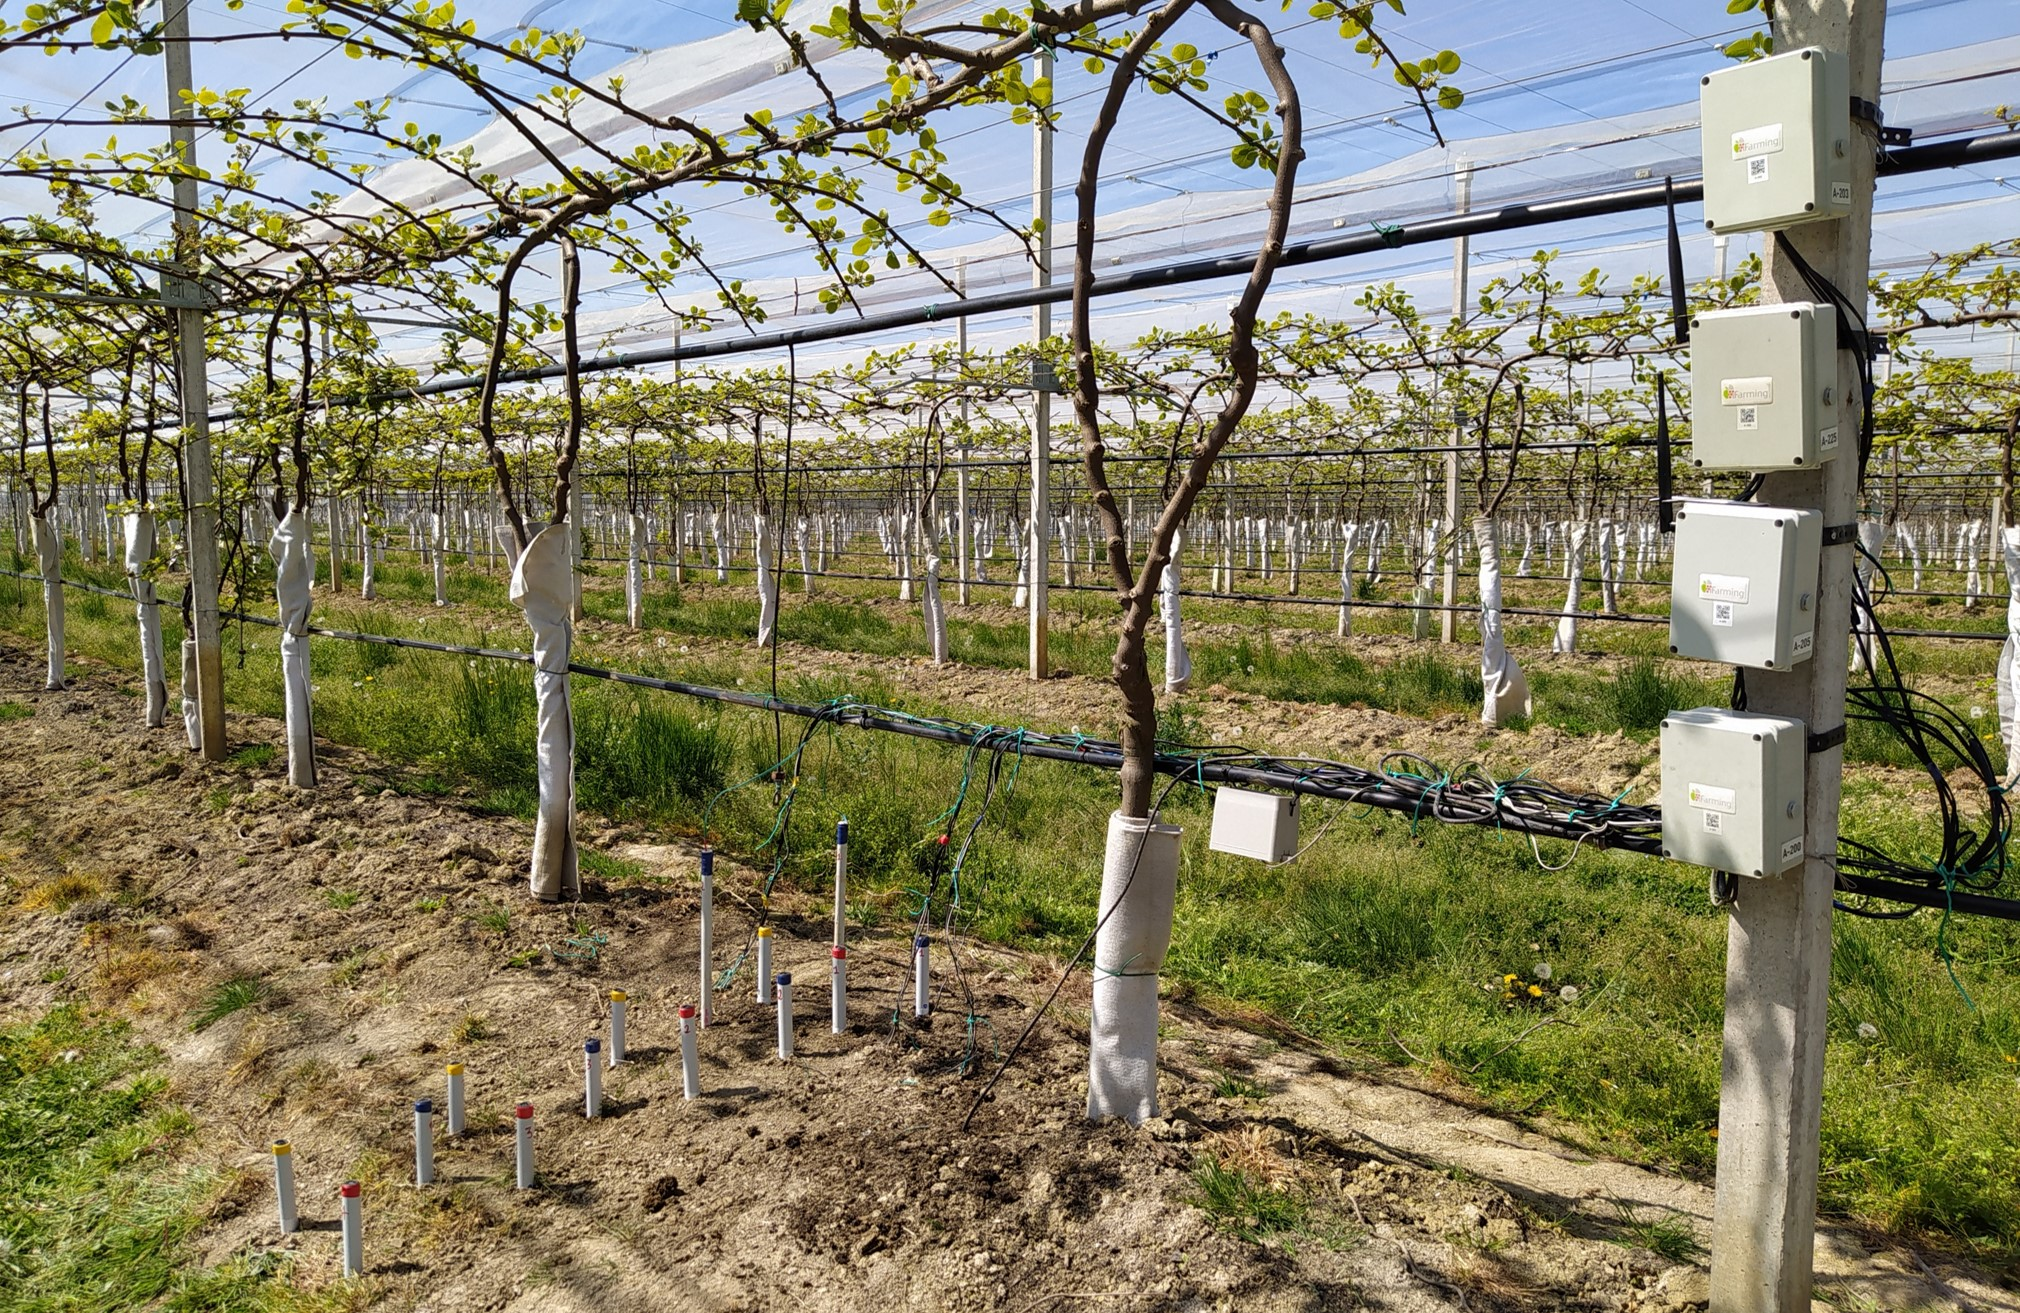
\includegraphics[scale=.4]{chapters/physics-aware/pluto/img/sensors.jpg}
    \end{subfigure}
    \caption{A sensor grid is monitoring soil moisture close to a kiwi tree near Faenza, Italy. The watering system is composed of single-pipeline drippers.}
    \label{pluto-fig:installation}
\end{figure}

Soil moisture varies continuously within the soil volume while the raw sensors provide point-wise measurements.
Furthermore, in most real-world applications, the number of sensors is by far less than those we used in our research project; this further reduces the comprehensiveness of the measurements.
For instance, companies involved in Agro.Big.Data.Science \cite{ABDS} relied on 1 to 3 sensors disposed at different depths (i.e., a 0D or a 1D grid).
The moisture profile, based on raw sensor measurements, estimates soil moisture of the whole soil volume at a fine-grained resolution.

\begin{definition}[Moisture profile]
Given an $n$-dimensional sensor grid $S$, the \emph{moisture profile} is an $n$-dimensional grid $P = \{p^1, ..., p^{|P|}\}$ that approximates, in each $p^i$, the soil moisture measured by $S$. $P$ is \emph{fine-grained} with respect to $S$ since $|P| > |S|$. 
\end{definition}

The approximation $p^i.v$ is assumed to be constant in the region surrounding $p^i$, whose granularity depends on $|P|$.

\begin{example}
Given a 2D sensor grid covering an area of $0.6 m^2$ (i.e., a rectangle with a width of $1m$ and a height of $0.6m$), we employed a sensor grid with 12 sensors (i.e., $|S| = 12$) and a moisture profile with 1000 points (i.e., $|P| = 1000$). As a result, we obtained a moisture profile having a granularity of $6 cm^2$ (i.e., $0.6 m^2 / 1000$) while the sensor grid granularity is $500cm^2$ (i.e., $0.6 m^2 / 12$). For the sake of clarity, \Cref{pluto-fig:moisture-sens} shows a sensor grid with $|S|=9$ and \Cref{pluto-fig:moisture-profile} shows a moisture profile with $|P|=25$.
\end{example}

A moisture profile covers the sensor grid region that is typically smaller, in size and dimensionality, than the soil volume. To provide a comprehensive estimation of the whole soil volume, we rely on the following assumption of \emph{symmetry}: the portions of the soil volume that are not covered by the sensor grid behave as the monitored one; in other words, the profile of the uncovered portions can be obtained under rotation or translation of the moisture profile.
\Cref{pluto-fig:symm} shows the symmetries in the case of 2D and 3D grids.
The symmetry assumption is verified for 2D grids when the drippers along a tree row are close enough to ensure homogeneous soil moisture.
If the distance between the drippers is high and the soil moisture along the row is not constant, a 3D grid must be adopted to satisfy the symmetry assumption.
Obviously, a 3D grid does not require any symmetry assumption if sensors are distributed all around the tree.
However, given a fixed amount of sensors, not exploiting the assumption of symmetry results in a coarser grid.

We emphasize that all the soil moisture estimation approaches based on sensors implicitly make symmetry assumptions: if a single sensor (0D installation \cite{arif2013estimation}) is used, the measured moisture is assumed as the reference value for the whole soil volume (i.e., it is assumed to be constant all over the soil volume); if a column of sensors (1D installation \cite{Karandish2016892, Goldstein2018421, Jimenez20201327, Pan2021, Li20152382}) is used the moisture is considered constant at a given depth. From this point of view, PLUTO's 2D and 3D grids progressively lighten such assumptions leading to a more accurate result. Obviously, some assumptions of symmetry remain, but they seem reasonable especially in the agricultural context: orchard rows are (or can be) built to be symmetrical. For example, the kiwi orchards involved in the Agro.Big.Data.Science project (i) were north-south oriented to have the same sun exposure on both the sides of the row; (ii) exploit a T-Bar training system; (iii) have a symmetric raised bed (i.e., with the same slope on both sides of the row).
More in general, to handle the variability within a single installation, it is always possible to design a grid layout that involves both sides of the row and, to handle variation within different parts of the field, two replicas can be installed.
In the following, \Cref{pluto-sec:FromSensorsToMoistureProfile} details the implementation of how switch from sensors to moisture profiles (i.e., via profiling functions), \Cref{pluto-sec} illustrates the visual components of PLUTO.

\begin{figure}[t]
\centering
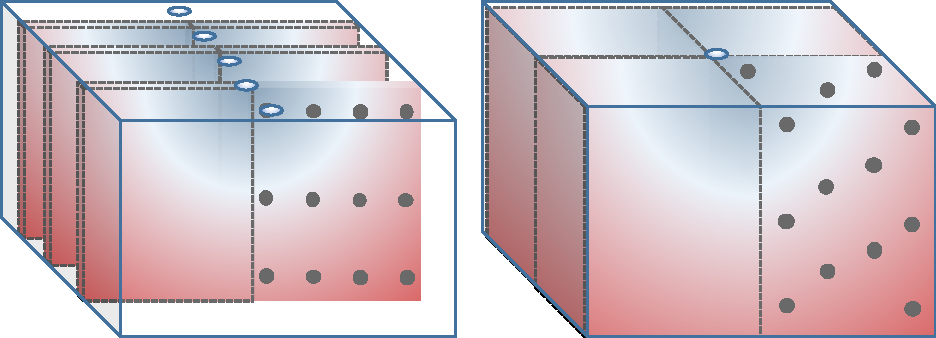
\includegraphics[scale=.6]{chapters/physics-aware/pluto/img/SensorGrid3.pdf}
\caption{Symmetries in watered soil: dotted rectangles (left) or parallelepipeds (right) replicate the data collected by the sensor grids.}
\label{pluto-fig:symm}
\end{figure}

\subsection{From Sensors to Moisture Profile}
\label{pluto-sec:FromSensorsToMoistureProfile}
The transformation of raw sensor measurements into a moisture profile is achieved through a profiling function. 
\begin{figure}[t]
\centering
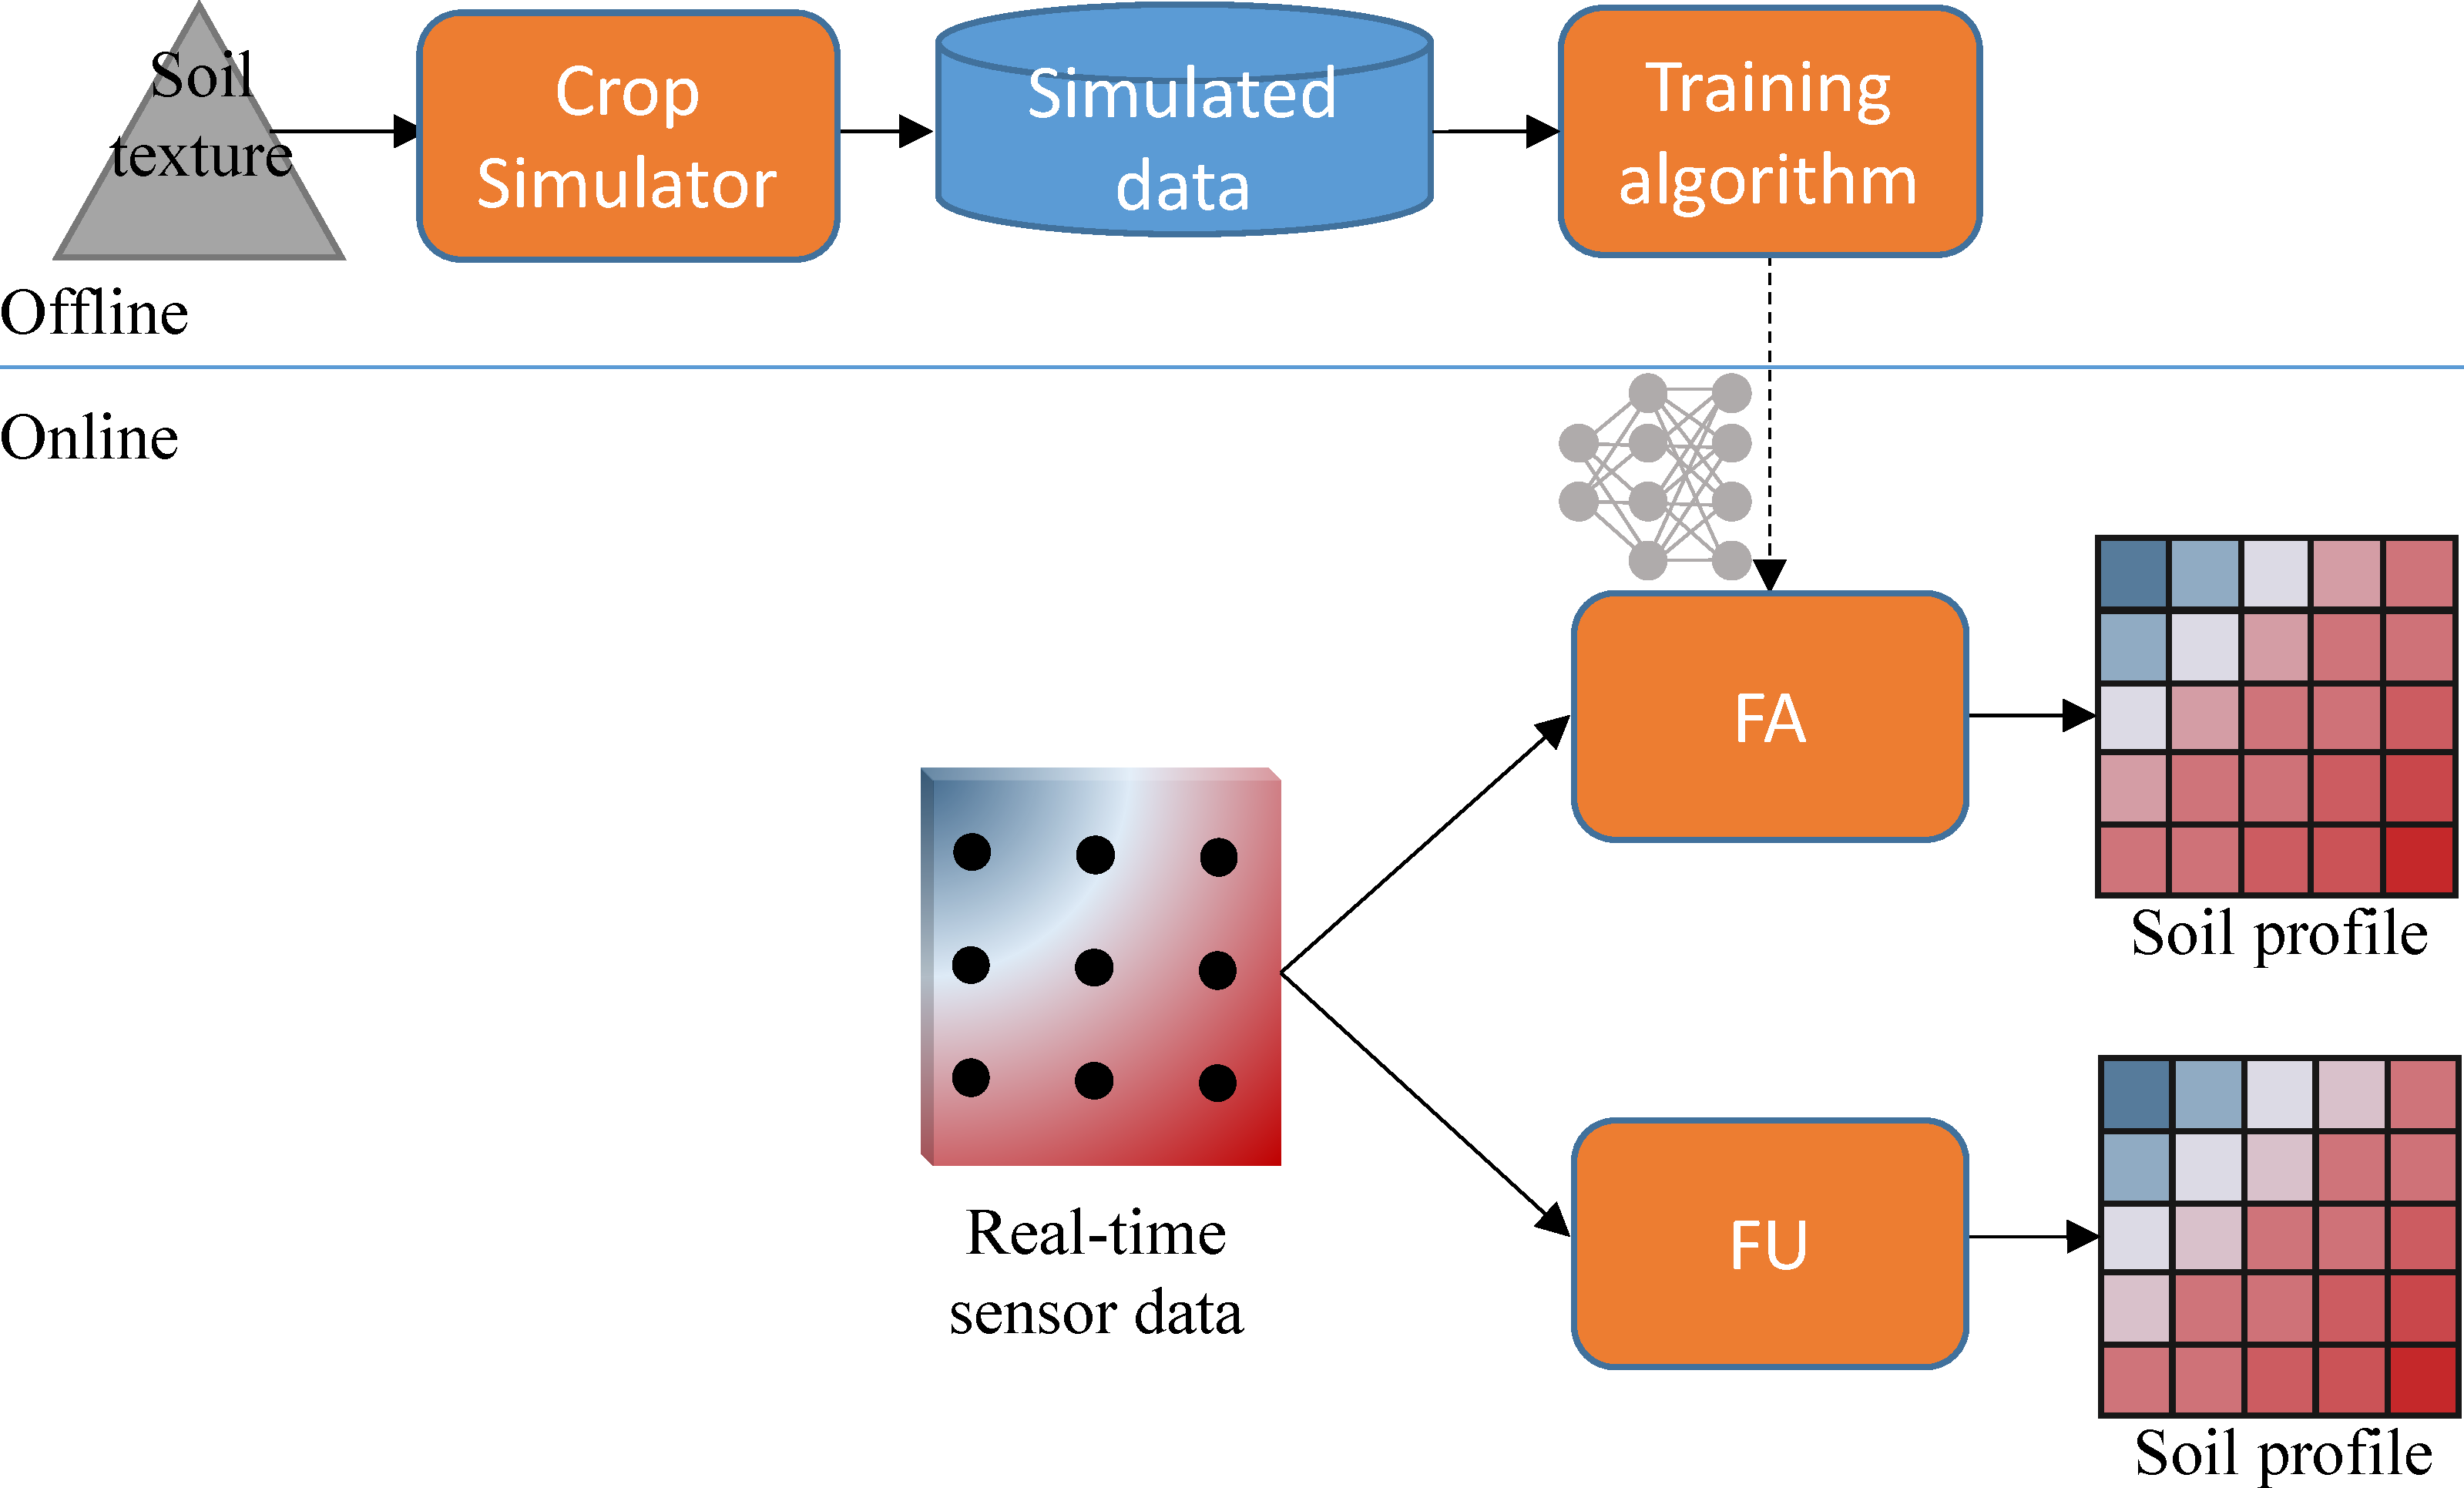
\includegraphics[scale=.2]{chapters/physics-aware/pluto/img/process.pdf}
\caption{Feature-aware and feature-unaware processes for building a moisture profile.}
\label{pluto-fig:process}
\end{figure}
\begin{definition}[Profiling function]
Given an $n$-dimensional sensor grid $S$ and a moisture profile $P$, a \emph{profiling function} $f : S \rightarrow P$ approximates the values of the moisture profile $P$ starting from the sensor grid $S$.
\end{definition}

The role of a profiling function is approximating the soil moisture values in those positions of the moisture profile where a sensor is not present. 
A profiling function is based on sensor grid measurements and can optionally exploit further information about the behavior of the soil. 
Several profiling functions can be adopted. 
We propose two alternative approaches that differ in the information exploited.
\begin{itemize}
    \item \emph{Soil-feature-unaware} - FU: exploits the sensor measurements only. The most obvious choice is to carry out a linear interpolation between pairs of sensor values.
    \item \emph{Soil-feature-aware} - FA: exploits the knowledge about soil hydrological dynamics to keep into account non-linearities and to get a more accurate estimation.
\end{itemize}

\Cref{pluto-fig:process} sketches the two alternative profiling functions and
% The feature-unaware function does not require to be fitted to a specific field and only gets sensor data as input, while the feature-aware function is trained offline to capture non-linear behaviors that result in a more accurate moisture profile.
\Cref{pluto-fig:FU_FA} exemplifies their main differences showing the profiles obtained by applying such functions to a grid of four sensors on the corners.
The values for the sensors are the same for the two profiles (top-left=-10cbar, top-right=-300cbar, bottom-left=-200cbar, bottom-right=-300cbar).
The profile on the left is obtained by applying the feature-unaware profile function, while the one on the right by applying the feature-aware function.
We note that the former has issues in capturing non-linearities in soil moisture dynamics; yet, we also emphasize that this is a worst-case scenario as our feature-unaware function also captures non-linear behaviors.
Indeed, using a grid of sensors, we are implicitly adopting a local regression approach \cite{loader2006local,cleveland1988locally}.
Although local regression approaches are bound to linear behavior between sensor pairs, the composition of several linear strokes can approximate a non-linear trend.
Conversely, our feature-aware function models the non-linearities between sensor pairs too.
The lower level of soil moisture in the upper right part results from the combination of two factors that are better captured via information wrt. the soil: this region (i) is proximal to the surface (thus it is more subject to atmospheric events) and (ii) belongs to the unwatered volume.
The gap between the two approximations grows as the distance between the sensors increases.

\subsubsection{Feature Unaware Profiling Function}

We rely on the well-known $n$-linear interpolation, where $n$ is the profile grid dimensionality.
For the sake of conciseness, in the following, we describe the $2$-linear case. 
Given a 2D sensor regular grid $S$, this technique carries out a linear interpolation in each dimension independently from each other.
The approach consists of two phases (\Cref{pluto-fig:statistical-profiling-function-explanation}).
For each point $p \in P$ of the moisture profile to be computed: (i) we find the four sensors $S$ that determine the minimum bounding rectangle enclosing $p$ (\Cref{pluto-fig:statistical-profiling-function}), then (ii) we compute $p.v$ (\Cref{pluto-fig:bilinear-interpolation}) by interpolating along the $x_1$ axis first. Then, exploiting the obtained points $r$  (blue dots), interpolation is performed along the $x_2$ axis and the value $p.v$ is finally determined.
Below follows the formal definition.

\begin{figure}[t]
\centering
\begin{subfigure}[t]{.45\textwidth}
\centering
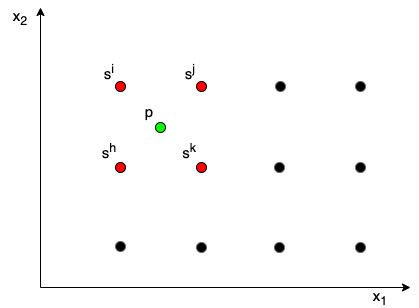
\includegraphics[scale=.4]{chapters/physics-aware/pluto/img/statistical_profiling_function.png}
\caption{Bounding rectangle for $p$}
\label{pluto-fig:statistical-profiling-function}
\end{subfigure}
~
\begin{subfigure}[t]{.45\textwidth}
\centering
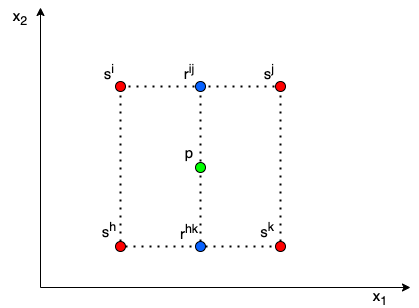
\includegraphics[scale=.4]{chapters/physics-aware/pluto/img/bilinear_interpolation.png}
\caption{Bilinear interpolation}
\label{pluto-fig:bilinear-interpolation}
\end{subfigure}
\caption{A 2D example of the feature-unaware function.}
\label{pluto-fig:statistical-profiling-function-explanation}
\end{figure}


\begin{align*}
    r^{ij}.v &= \frac{s^j.x_1-r^{ij}.x_1}{s^j.x_1-s^i.x_1} s^i.v + \frac{r^{ij}.x_1-s^i.x_1}{s^j.x_1-s^i.x_1} s^j.v\\
    r^{hk}.v &= \frac{s^k.x_1-r^{hk}.x_1}{s^k.x_1-s^h.x_1} s^h.v + \frac{r^{hk}.x_1-s^h.x_1}{s^k.x_1-s^h.x_1} s^k.v \\
    p.v &= \frac{r^{ij}.x_2-p.x_2}{r^{ij}.x_2-r^{hk}.x_2} r^{hk}.v + \frac{p.x_2-r^{hk}.x_2}{r^{ij}.x_2-r^{hk}.x_2} r^{ij}.v
\end{align*}
The trilinear procedure is analogous: it just has three steps instead of two.


\subsubsection{Feature Aware Profiling Function}
The feature-aware function captures non-linear soil moisture behaviors by exploiting the knowledge about the hydrological fluxes. To this end, we rely on an Artificial Neural Network (ANN), a ML model, that returns the estimated values for each profile point after learning the soil behavior from the data generated by CRITERIA \cite{Bittelli2011253}, a process-based model.
%\jgc{}{The ANN profiling function,} Given the sensor measurements, \jg{we leverage an Artificial Neural Network (ANN)} that returns the estimated values for each profile point.
The learning process is sketched in \Cref{pluto-fig:process}.
The ANN learns the soil behavior from simulated data in an off-line phase, which is carried out only once at the time of installation of the system.
%We rely on a \jg{crop simulation model??} \cite{Bittelli2011253}  to create the training dataset.
CRITERIA reproduces hydrological fluxes in the soil volume implementing Richard's equations.
The simulator models the following elements of the soil volume: (i) the soil texture; (ii) the shape of the tree roots; (iii) the watering system type and layout; and (iv) the sensor layout.
Such data are provided as input by the farmer.
Then, training data are generated running the simulator according to simulated weather conditions and watering sessions.
Generating hourly data over a 4-month period proved to be sufficient to train the ANN.

ANNs have been chosen for the feature aware profiling function due to the following properties:
\begin{itemize}
    \item Low resource consumer: once trained offline, the ANNs are fast and require limited computational resources. 
    \item Powerful \& Flexible: can provide accurate profiles (i.e., they properly capture non-linearities) even though the grid layout includes a limited number of sensors. 
    \item Robust: ANNs are well-known to work well even in case of dirty or missing data. This may happen when a sensor occasionally fails to provide the correct data. 
\end{itemize}

\begin{table}[t]
\centering
\caption{The ANN hyper-parameter configuration retrieved by HyperOpt.}
% \scriptsize{
\begin{tabular}{lc}
\hline
Hyper-parameter & Value \\ \hline
\# Hidden Layers & 1 \\
\# Neurons per layer & 100 \\
Activation function & Tanh \\
Normalization & Z-score \\
\# Training epochs & 50 \\
Batch size & 30 \\
Reduce learning rate & factor=2, patient=10 \\ \hline
\end{tabular}
% }
\label{tab:ann_configuration}
\end{table}

\Cref{tab:ann_configuration} reports the hyper-parameters for the PLUTO ANN.
We adopted a feed forward ANN (i.e., neurons in the layers are connected without creating any cycle) with one, fully connected, hidden layer.
The input layer has one neuron for each sensor, the hidden layer has a hundred of neurons activated through the hyperbolic tangent activation function (e.g., values of the neurons are mapped according to the homonym mathematical function), and the output layer has as many neurons as the number of points in $P$ (see \Cref{pluto-fig:ANN}).
As to the learning hyper-parameters, the process involves 50 epochs, a batch size of 30 samples, and the learning rate (i.e., the step size towards the final solution) is reduced by a factor of 2 when no improvement is seen for a \textit{patient} number of 10 epochs.
%The neurons are activated through the hyperbolic tangent activation function.
Besides, a Z-score normalization (i.e., transforming data into a Gaussian distribution with mean 0 and standard deviation 1) is applied to the input values before feeding the network. This is due to the following reasons.
\begin{figure}[t]
\centering
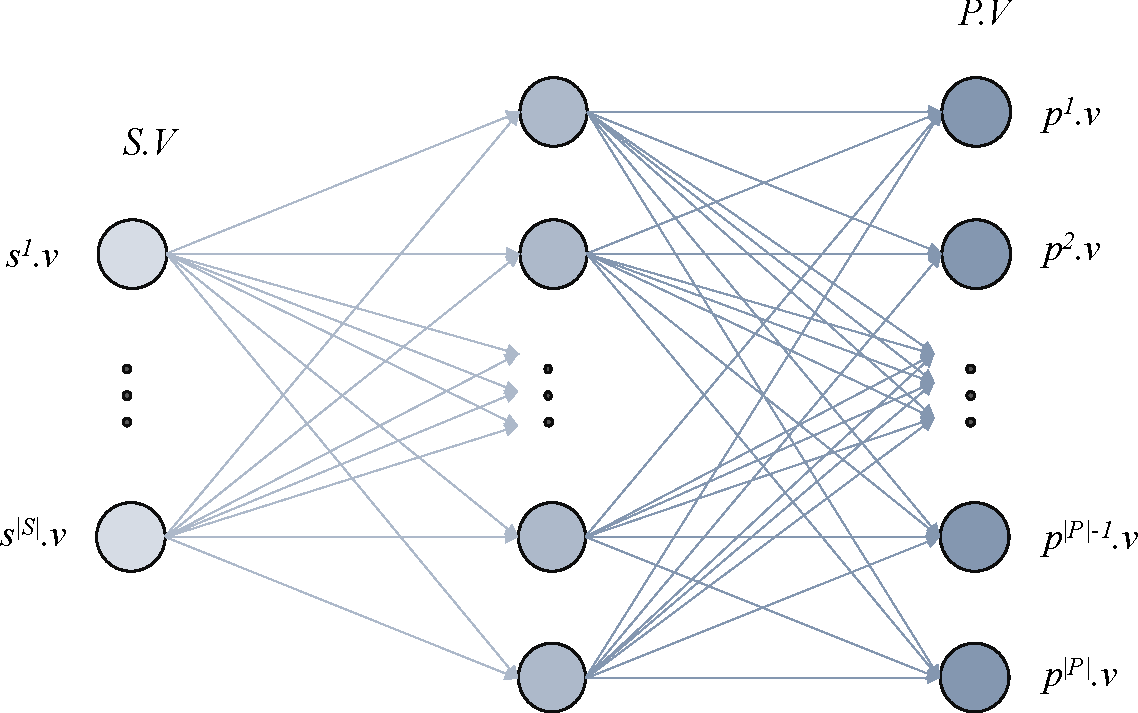
\includegraphics[scale=.4]{chapters/physics-aware/pluto/img/ANN.pdf}
\caption{The layout of the ANN profiling function.}
\label{pluto-fig:ANN}
\end{figure}

\begin{itemize}
    \item To give all the input values the same importance. Even though the soil moisture varies everywhere in the same range, we noticed sensible variations depending on the location of the sensor (e.g., the area right under the dripper and the opposite corner).
    \item To address ANN-specific training issues. Normalizing the inputs reduces the chances of getting stuck in local optima (e.g., balance the rate at which the ANN learns) and makes training faster (e.g., avoid the saturation of non-linear activation function).
\end{itemize}

All the hyper parameters (i.e., ANN strucure and learning rates) have been set through a hyper-parameter tuning process implemented with HyperOpt \citep{bergstra2015hyperopt}. HyperOpt exploits state-of-the-art optimization techniques to heuristically explore the huge search space of hyper-parameters. The adoption of a training set including several different weather conditions and watering sessions avoids overfitting (i.e., a learning process that returns a network that works well just for the specific cases it was trained for).


\begin{figure}[t]
\centering
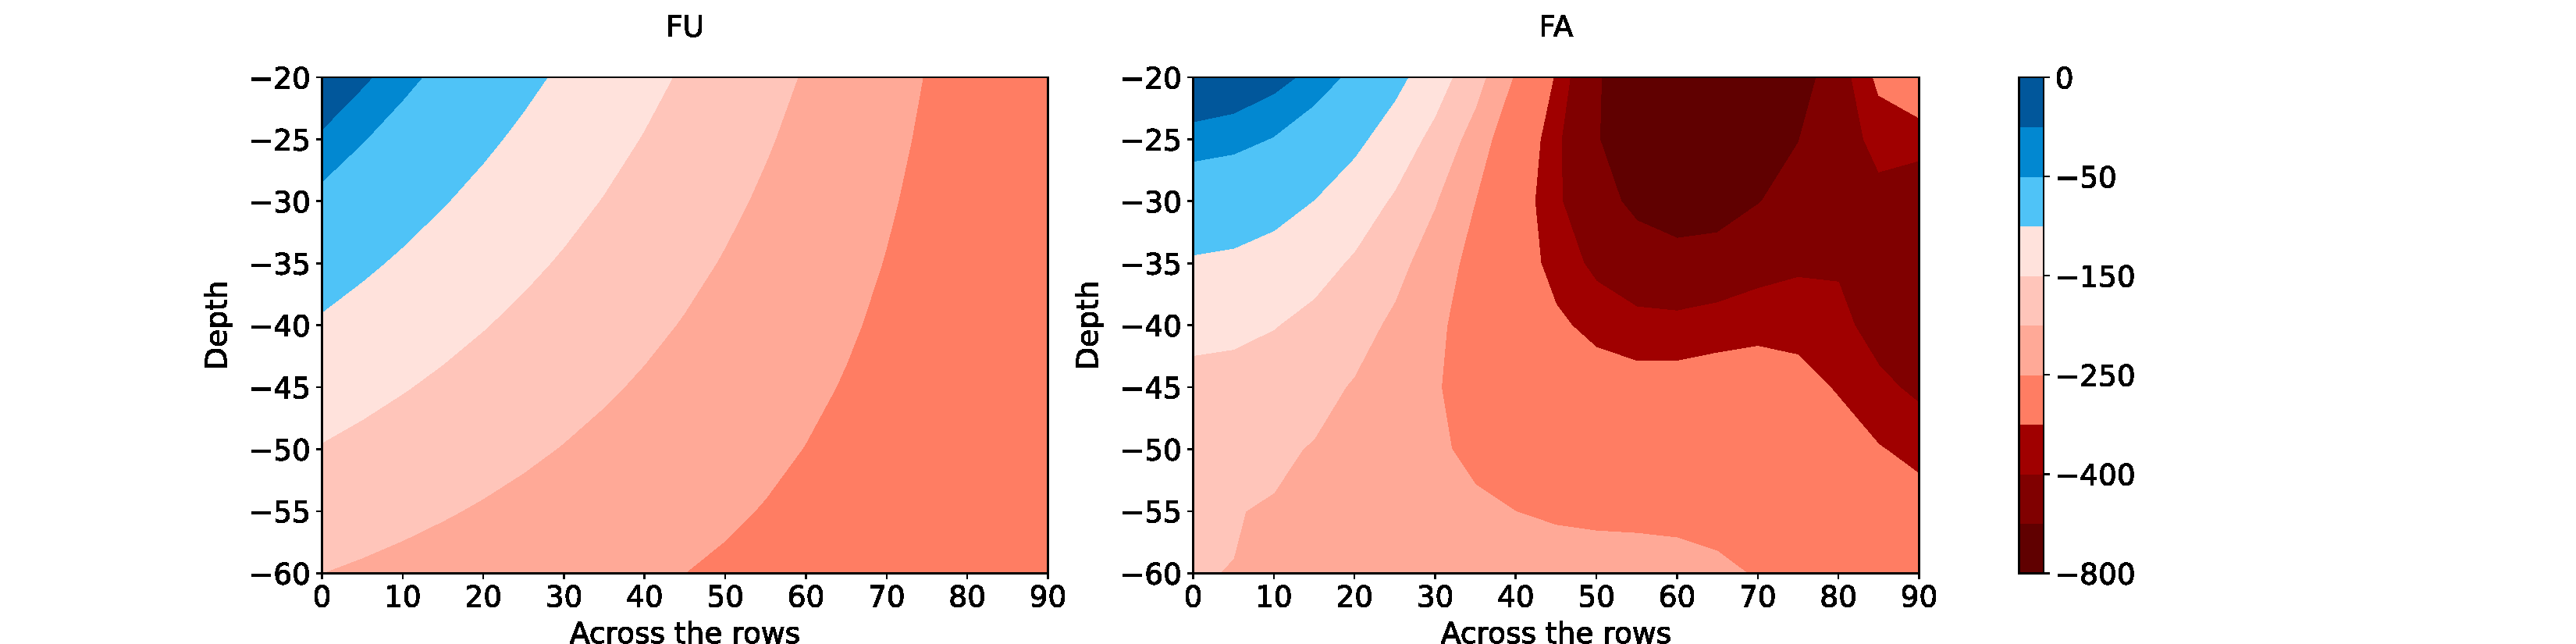
\includegraphics[scale=.25]{chapters/physics-aware/pluto/img/countor_plot.pdf}
\caption{Moisture profile built by the two types of profiling functions, namely feature-unaware (left) and feature-aware (right).}
\label{pluto-fig:FU_FA}
\end{figure}

\subsection{Visualization}
\label{pluto-sec:visualization}
Visualization allows easy exploitation of the moisture profile, enabling effective soil moisture monitoring.
We propose two visual components selected according to the data types and the following visualization goals \cite{golfarelli2020model}.
\begin{itemize}
    \item \emph{Historical soil moisture trend}: shows the variation of moisture over time.
    Independently of the profile dimensionality, a 2D stacked area chart is adopted.
    No spatial information is shown here.
    \item \emph{Spatial soil moisture}: shows the spatial distribution of soil moisture at a specific time. A 2D heat map or a 3D scatter plot is adopted depending on the profile dimensionality.
\end{itemize}
The two components are linked through \emph{interactive zooming} \cite{keim2002information}. When the user selects a specific time on the historical soil moisture trend, the corresponding spatial soil moisture at the time is shown.

Since the goal is to check that an ideal moisture profile is maintained, we define five crop-specific soil moisture ranges, each associated with a different color.
For our case of study on kiwi-trees \cite{ABDS}, Dark blue (in $[0, -30)$ cbar) and light blue (in $[-30, -100)$ cbar) show heavily/slightly portions of over-watered soil. Salmon pink (in $[-100, -300)$ cbar) represents the ideal case \cite{miller1998effects}.
Finally, light red (in $[-300, -1500)$ cbar) and dark red (in the range of $[-1500, -\infty)$ cbar) show slightly/heavily portions of under-watered soil.

\begin{figure}[t]
\centering
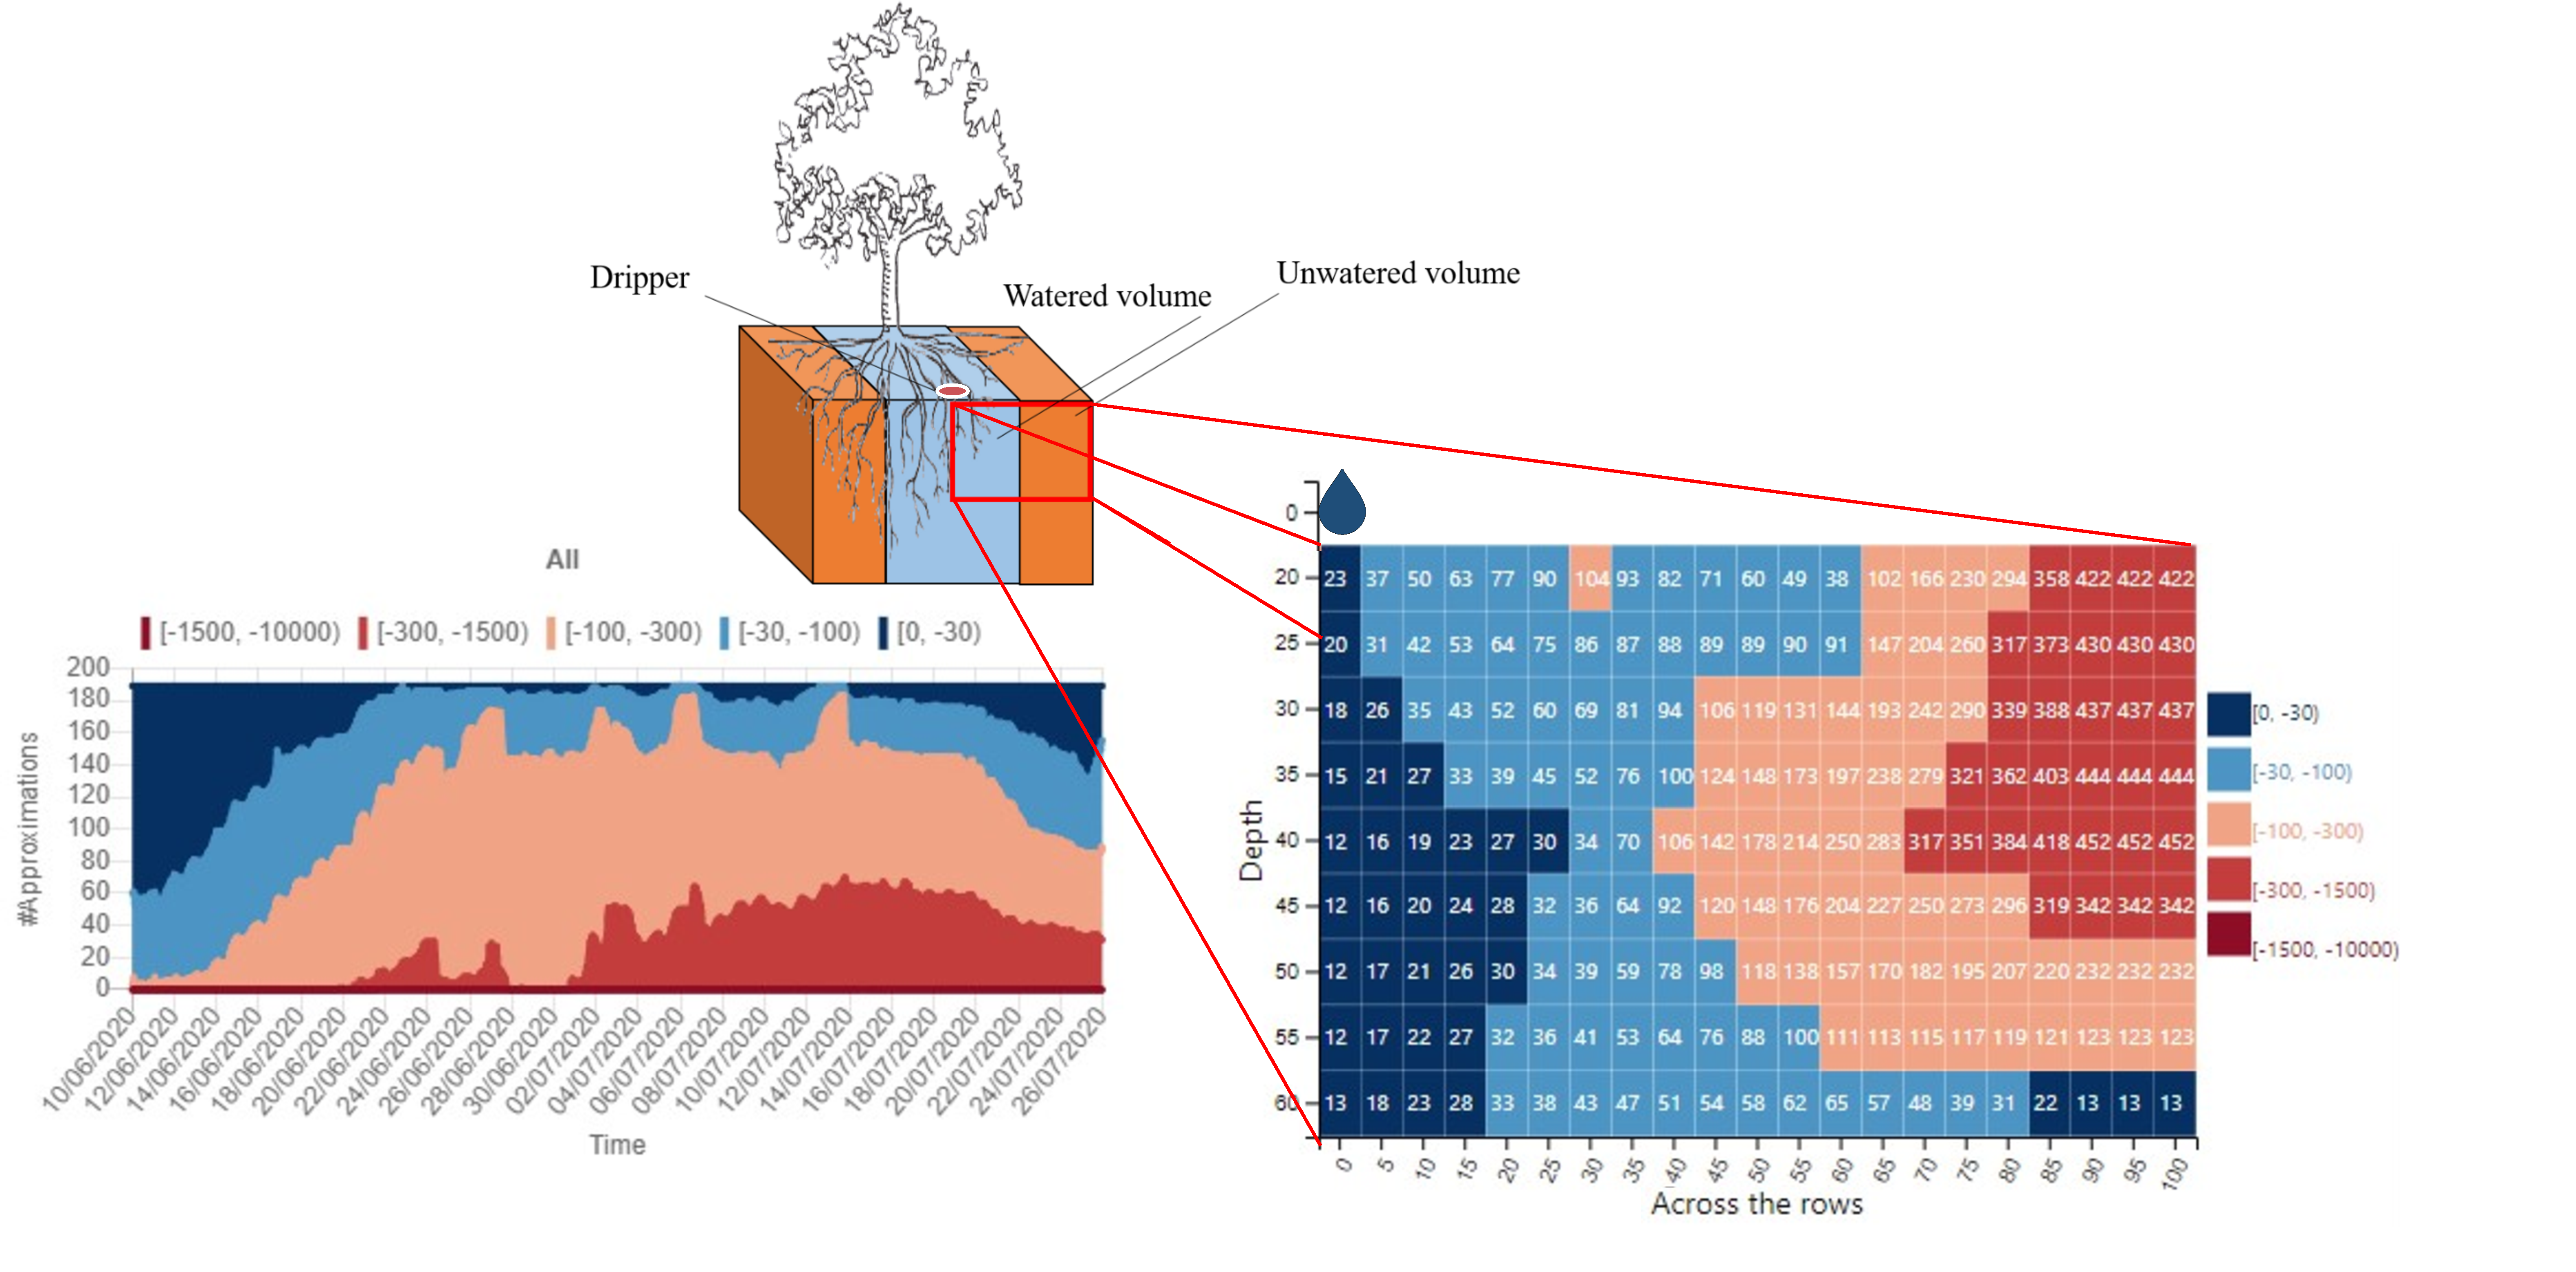
\includegraphics[scale=.12]{chapters/physics-aware/pluto/img/2d-visualization.pdf}
% \caption{A 2D-visualization example.}
\caption{Visualization of a 2D profile: (left) the historical soil moisture and (right) a snapshot of the spatial soil moisture. The rightmost legend shows the soil moisture ranges. The drop at depth $0$ represents the \textit{Dripper} position and the rightmost legend shows the soil moisture ranges.}
\label{pluto-fig:2D-visualization}
\end{figure}

\Cref{pluto-fig:2D-visualization} shows examples of historical soil moisture trend and spatial soil moisture charts for a 2D profile.
The historical soil moisture chart shows how the soil gradually dries out during the dry season.
In May the soil is mostly wet, while in June the first irrigations are necessary. 
Also, note how the single pipeline dripper fails to eliminate the red area due to the presence of an unwatered region in the soil volume.
For the chosen zoom date, the spatial soil moisture chart shows the moisture profile in detail. Each cell corresponds to a profile element.
The following areas can be highlighted: (i) the region under the dripper where the effects of irrigation are apparent; (ii) the superficial portion away from the dripper that is very dry as it is not irrigated; and (iii) the deep region which is less affected by atmospheric agents and in which constant soil moisture remains regardless of the effects of watering.
The profile highlights how the soil moisture spreads laterally thanks to the combined effect of the roots and the permeability characteristics of the soil.

\begin{figure}[t]
\centering
\begin{subfigure}[t]{.45\textwidth}
\centering
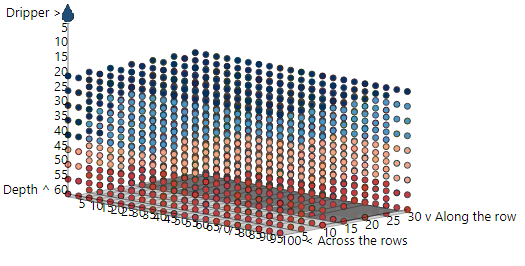
\includegraphics[scale=.4]{chapters/physics-aware/pluto/img/3d-visualization-a.png}
\end{subfigure}
~
\begin{subfigure}[t]{.45\textwidth}
\centering
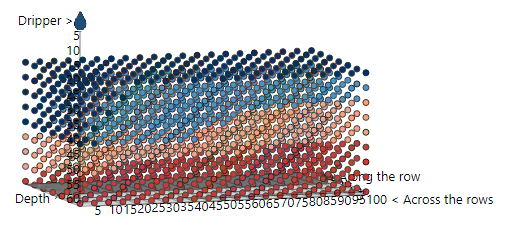
\includegraphics[scale=.45]{chapters/physics-aware/pluto/img/3d-visualization-b.png}
\end{subfigure}
% \caption{A 3D visualization during a rotation.}
\caption{Visualizing rotations of a 3D profile.}
\label{pluto-fig:3D-visualization}
\end{figure}

\Cref{pluto-fig:3D-visualization} shows an example of a 3D spatial soil moisture chart.
Each sphere corresponds to a profile element. The colors are the same as in the 2D visualization.
Spaces between spheres allow the inner side of the 3D profile to be explored. Furthermore, to facilitate the analysis, the chart can be rotated along the three axes. 
The soil moisture gradient along the third dimension (i.e., along the row) is better highlighted by the third orientation of the chart and justifies the adoption of a 3D profile.

Starting from the spatial profile, we derive many meaningful visualizations. \Cref{pluto-fig:variazione-umidita-profilo}-left shows the profile variance chart, which reports the soil moisture variance in a given period.
The lighter areas are those where soil moisture varies the most. Similarly, \Cref{pluto-fig:variazione-umidita-profilo}-right shows the profile average chart which reports the average soil moisture in a given period.
The charts are designed to support the work of both agricultural technicians and farmers. For example, in the Agro.Big.Data.Science projects the main questions posed by such users were:
\begin{itemize}
    \item \emph{What is the watered volume?}:
    this region is typically characterized by two phenomena: high moisture and high suction by the roots.
    Depending on the supplied quantity of water, the summation of the two phenomena determines different effects.
    In the case of over-watering, the watered volume remains always wet, with high values in the average chart and low values in the variance chart as the roots and the atmospheric phenomena are not able to absorb the water.
    Conversely, in the case of correct irrigation, the average chart shows medium values while the variance one shows high values mainly due to the suction made by the roots. This is the case for \Cref{pluto-fig:variazione-umidita-profilo}. 
    \item \emph{Where is the root suction higher?}: 
    a high root suction quickly reduces the moisture in the soil and results in a strong soil moisture variance. 
    \item \emph{How soil moisture dynamics impact on the watered volume?}: if, after increasing the quantity of water supplied to the soil, the watered volume does not increase significantly, then the soil disperses water in depth due to its characteristics.
\end{itemize}
In the context of the Agro.Big.Data.Science project agricultural technicians and some \emph{data enthusiast farmers} \cite{morton2014support} already had the competences to directly exploit the charts, while most of the farmers had been trained. We strongly believe that the progressive digitization in agriculture will drive all farmers to take advantage of these solutions, as it has already happened to operators in other industries.

A demo of the PLUTO visualization system is available at \url{https://big.csr.unibo.it/projects/pluto}. The monitoring system can be completed by the following information collected through a weather station and a water meter:
\begin{itemize}
    \item a single line chart showing the max/min/avg air temperature;
    \item a bar chart showing the mm of rain that fell each day;
    \item a bar chart showing the mm of water supplied, each day, through watering. 
\end{itemize}
Although the role of data processing and visualization is often overlooked, such visualizations contribute to a comprehensive understanding of the evolution of the profile.

\begin{figure}[t]
\centering
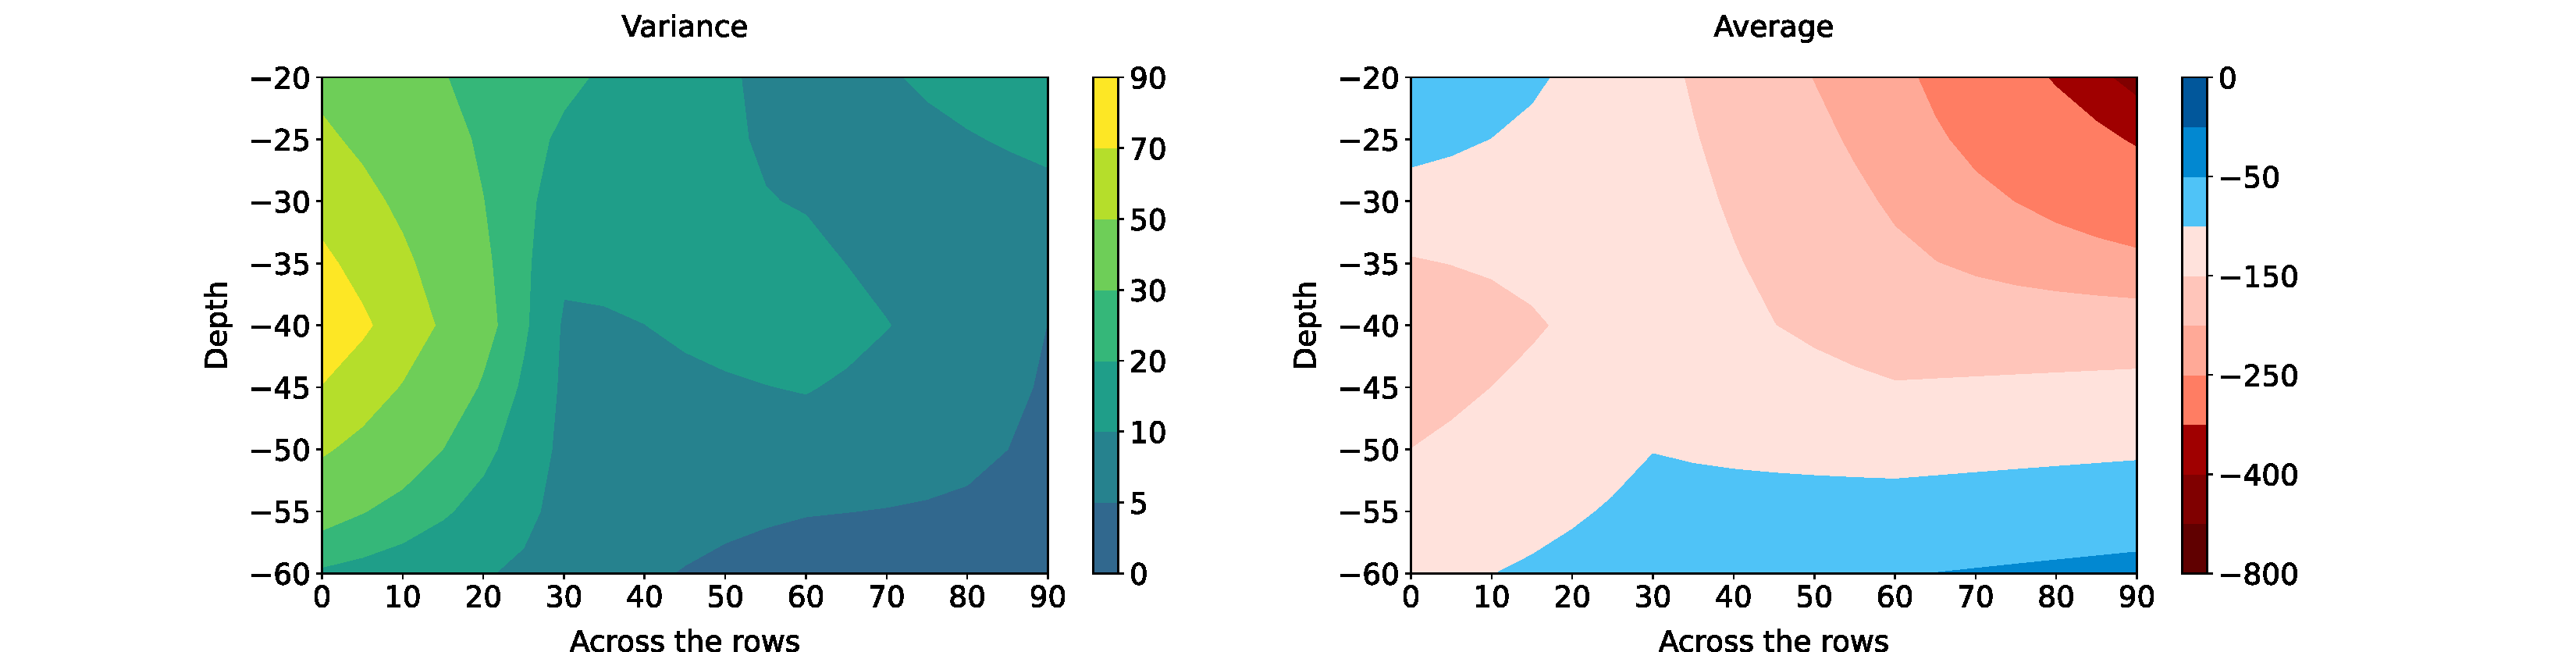
\includegraphics[scale=.25]{chapters/physics-aware/pluto/img/countor_plot_std_mean.pdf}
\caption{Soil moisture variance (left) and average (right) in cbar along a 1-week period; the orchard is watered through a single-pipeline dripper system.}
\label{pluto-fig:variazione-umidita-profilo}
\end{figure}

\section{Results and Discussion}
\label{pluto-sec:ResultsAndDiscussion}
We tested PLUTO on the installations of the Agro.Big.Data.Science project \cite{ABDS}.
Data have been collected in the irrigation season from May to September in 2020 and 2021.
Installations are taken from two orchards: one in the plains and one in the hills around Faenza, in the province of Ravenna, Italy.
The orchards were planted in 2010 as a self-rooting Hayward variety (A. chinensis var deliciosa), grafted in 2012 with Gold 3 (A. chinensis var chinensis). 
Kiwifruit vines were spaced 2m along the row and 4.5m across the rows.
Different irrigation systems and sensor grid layouts have been considered as shown in \Cref{pluto-tbl:implants}.
Sensor data are sampled and collected every 15 minutes. 
% Please add the following required packages to your document preamble:
% \usepackage{booktabs}
\begin{table}[t]
\centering
% \footnotesize{
\begin{tabular}{@{}ccccccc@{}}
\toprule
Location & \# Grids & Grid Layout & \# sensors & Watering system \\ \midrule
Hilly & 1 & 3D & 15 & Single pipeline \\
Hilly & 2 & 2D & 12 & Single pipeline \\
Hilly & 2 & 2D & 12 & Double pipeline \\
Plain & 4 & 2D & 12 & Single pipeline \\ \bottomrule
\end{tabular}
% }
\caption{Description of the experimental implants.}\label{pluto-tbl:implants}
\end{table}

We emphasize that the number of sensors we use is much higher than necessary, as we will show below. 
Grids with 12-15 sensors were used to build the ground truth to carry out the tests. In each test only a subset of the available sensors was used to compute the profile, while the remaining ones were used as ground truth. In other words, we verify how well the profile approximates the soil moisture in positions where the real soil moisture is known to the tester but hidden to PLUTO. Profile accuracy is calculated as the Root Means Square Error (RMSE) between the ground truth sensor values and the values estimated by the profile. Obviously, the RMSE is computed only for those sensors that are not used to compute the profile.

\subsection{Accuracy Evaluation}
\label{pluto-sec:ApproachEvaluation}
\Cref{pluto-fig:2Dperformance} shows the system performance, for the 2D profile, varying the number of input sensors. Tests have been repeated for all the available installations.
To better understand the advantage provided by PLUTO, we also highlighted the performance of profiling based on a single sensor --- 0D setting --- (i.e., the \emph{de facto} standard) or a column of 3 sensors at different depths --- 1D setting. 
To extend the soil moisture value of the single sensor to the entire soil volume, we must assume the soil moisture to be constant in the whole volume. 
Similarly, when a column of sensors is available, we assume that soil moisture is constant at the same depth in the soil.
Since the accuracy varies based on the sensor location, we choose the single sensor position (or the sensor line) that minimizes the RMSE as a fair comparison baseline.
The same methodology was adopted to displace the sensors used to calculate the profile. 
We refer to section \Cref{pluto-sec:sensors_disposal_evaluation} for an in-depth analysis of the layout of the profile sensors and the robustness of the system.

The 0D setting estimations are by far less accurate than the ones obtained by our profiling functions; indeed, three sensors are sufficient to halve its RMSE using the feature-aware profiling function. 
The 1D setting achieves slightly better results since it captures soil moisture at different soil depths, but fails in capturing longitudinal variations. 
The extent of these errors is not negligible since the optimal range for soil moisture for kiwi cultivation is $[-100;-300)$ cbar \cite{miller1998effects}.

RMSE for feature-aware and feature-unaware gradually decreases as the number of sensors increases. 
Note that the bilinear profiling function can be computed only for some sensor layouts, due to the intrinsic geometrical constraints (i.e., the profile region must be partitioned in bounding rectangles/cubes). 
The ANN profiling function always outperforms the bilinear one due to its capability to better model non-linear behaviors. 
This supremacy is more evident when the number of sensors is limited and the intra-sensor distances are larger (see \Cref{pluto-fig:FU_FA}). 
\begin{figure}[t]
\centering\
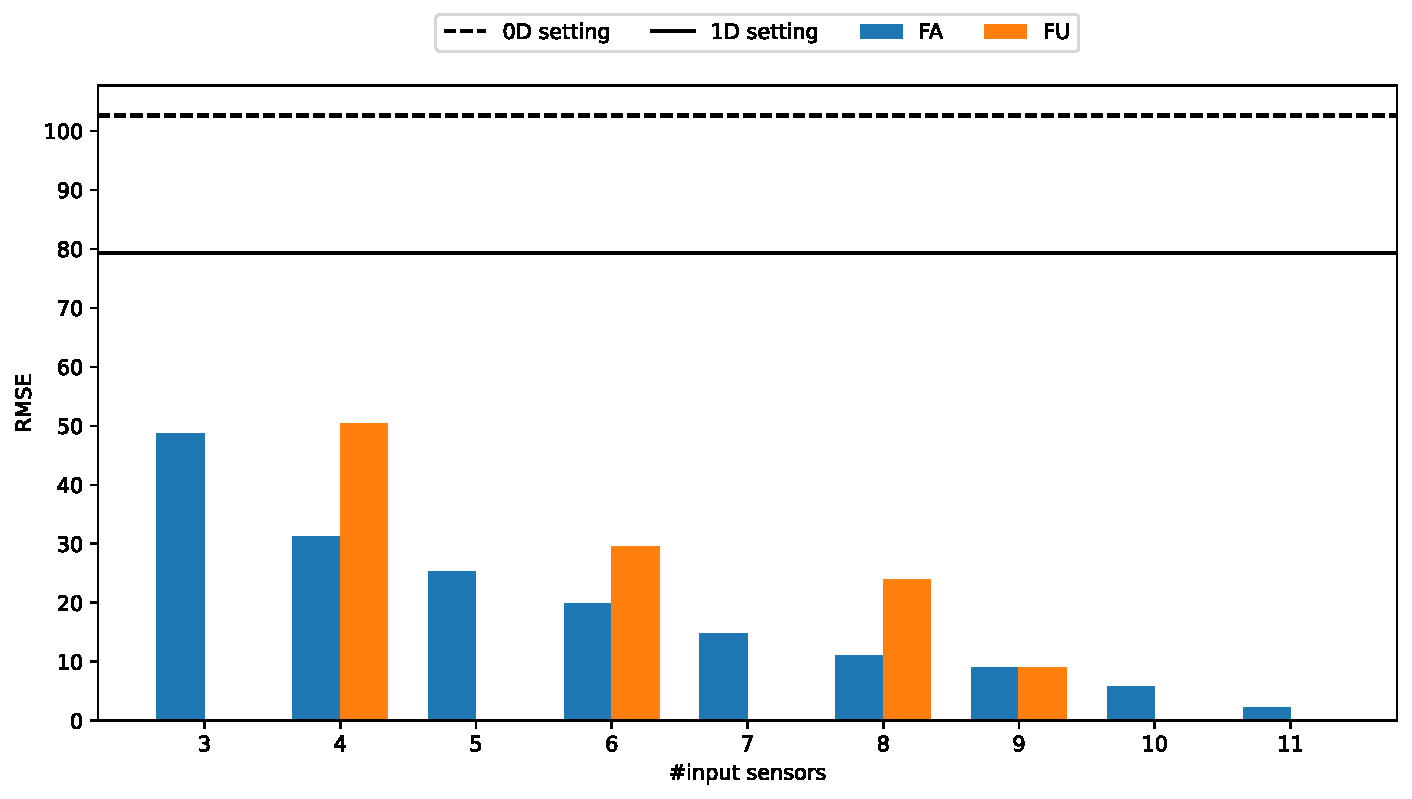
\includegraphics[scale=.5]{chapters/physics-aware/pluto/img/bar_plot.pdf}
\caption{2D profile performances as a function of the input  sensors. Single sensor (0D) and column (1D) settings are reported for comparison. }
\label{pluto-fig:2Dperformance}
\end{figure}

\begin{figure}[t]
\centering\
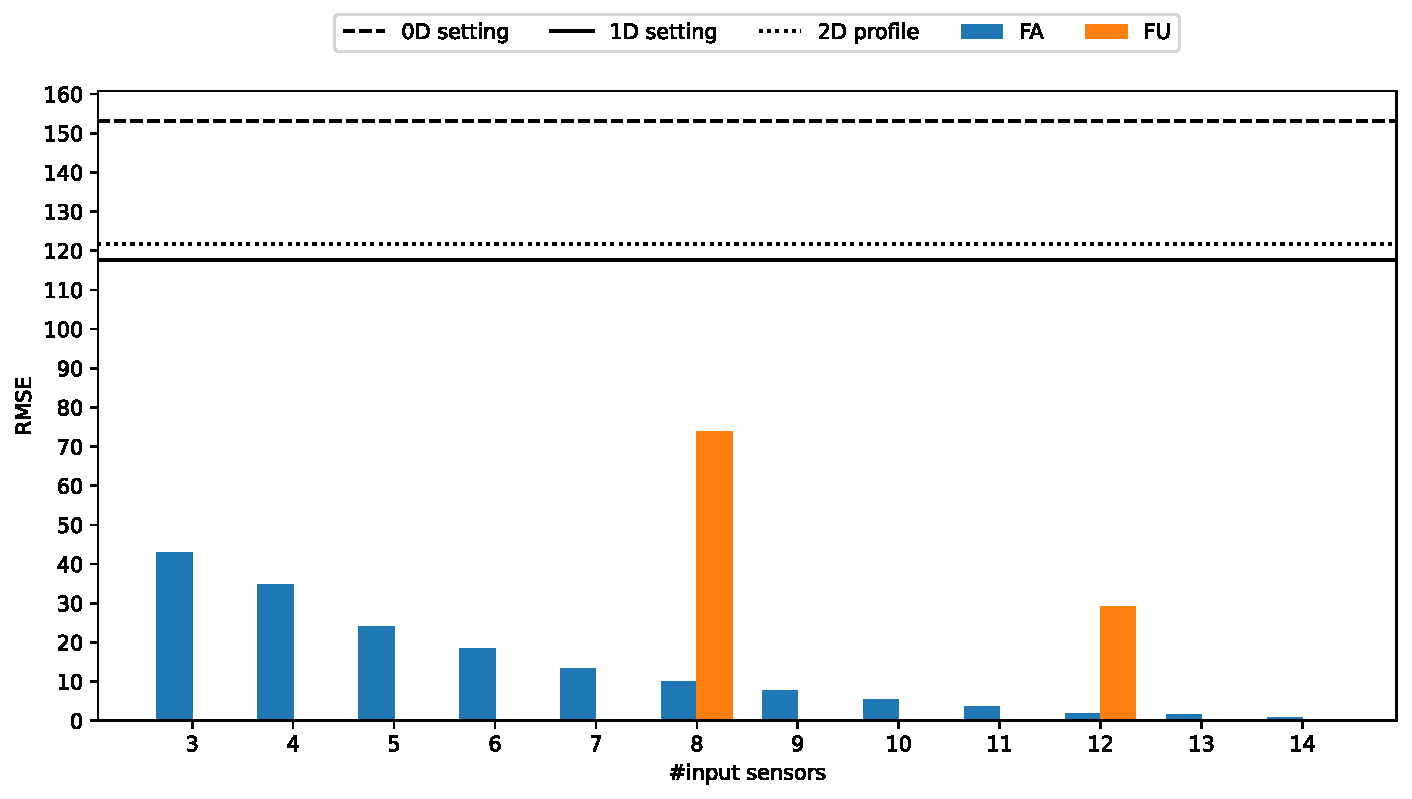
\includegraphics[scale=.5]{chapters/physics-aware/pluto/img/3d_bar_plot.pdf}
\caption{3D profile performances as a function of the input  sensors. Single sensor (0D), column (1D) settings, and (2D) profile are reported for comparison.}
\label{pluto-fig:3Dperformance}
\end{figure}

3D profile performances are reported in \Cref{pluto-fig:3Dperformance}. This type of profile measures soil moisture variability along the row, while 2D profiles assume soil moisture to be constant along the row. 
The chart shows that the assumption is partially true since the RMSE for the 2D profile (i.e., the dotted line) is higher than those related to the 3D ones. 
The RMSE further increases for the 0D and 1D settings as they progressively make stronger assumptions about symmetry. 
As expected, the RMSE for the 3D profiles decreases as the number of sensors increases, and the feature-aware profiling function overcomes the feature-unaware one.

%\begin{figure}[t]
%\centering
%\begin{subfigure}[t]{.4\textwidth}
%\centering
%\includegraphics[scale=.45]{chapters/physics-aware/pluto/img/single-pipe-2.pdf}
%\end{subfigure}
%~
%\begin{subfigure}[t]{.4\textwidth}
%\centering
%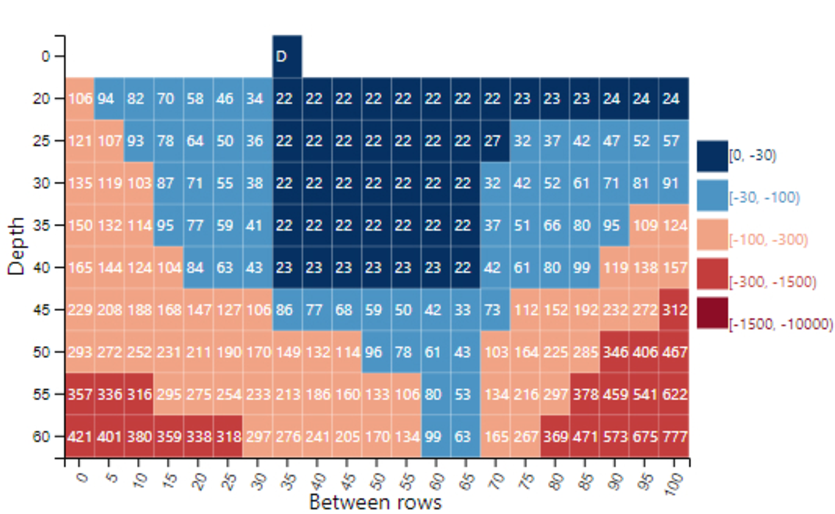
\includegraphics[scale=.45]{chapters/physics-aware/pluto/img/double-pipe.pdf}
%\end{subfigure}
%\caption{Profile comparison for orchards equipped with single pipeline dripper (left) and double pipeline dripper (right) watering systems. The cell labeled with letter \emph{D} at depth $0$ shows the \textit{Dripper} position.}
%\label{pluto-fig:pipeline-comparison}
%\end{figure}
\begin{figure}[t]
\centering\
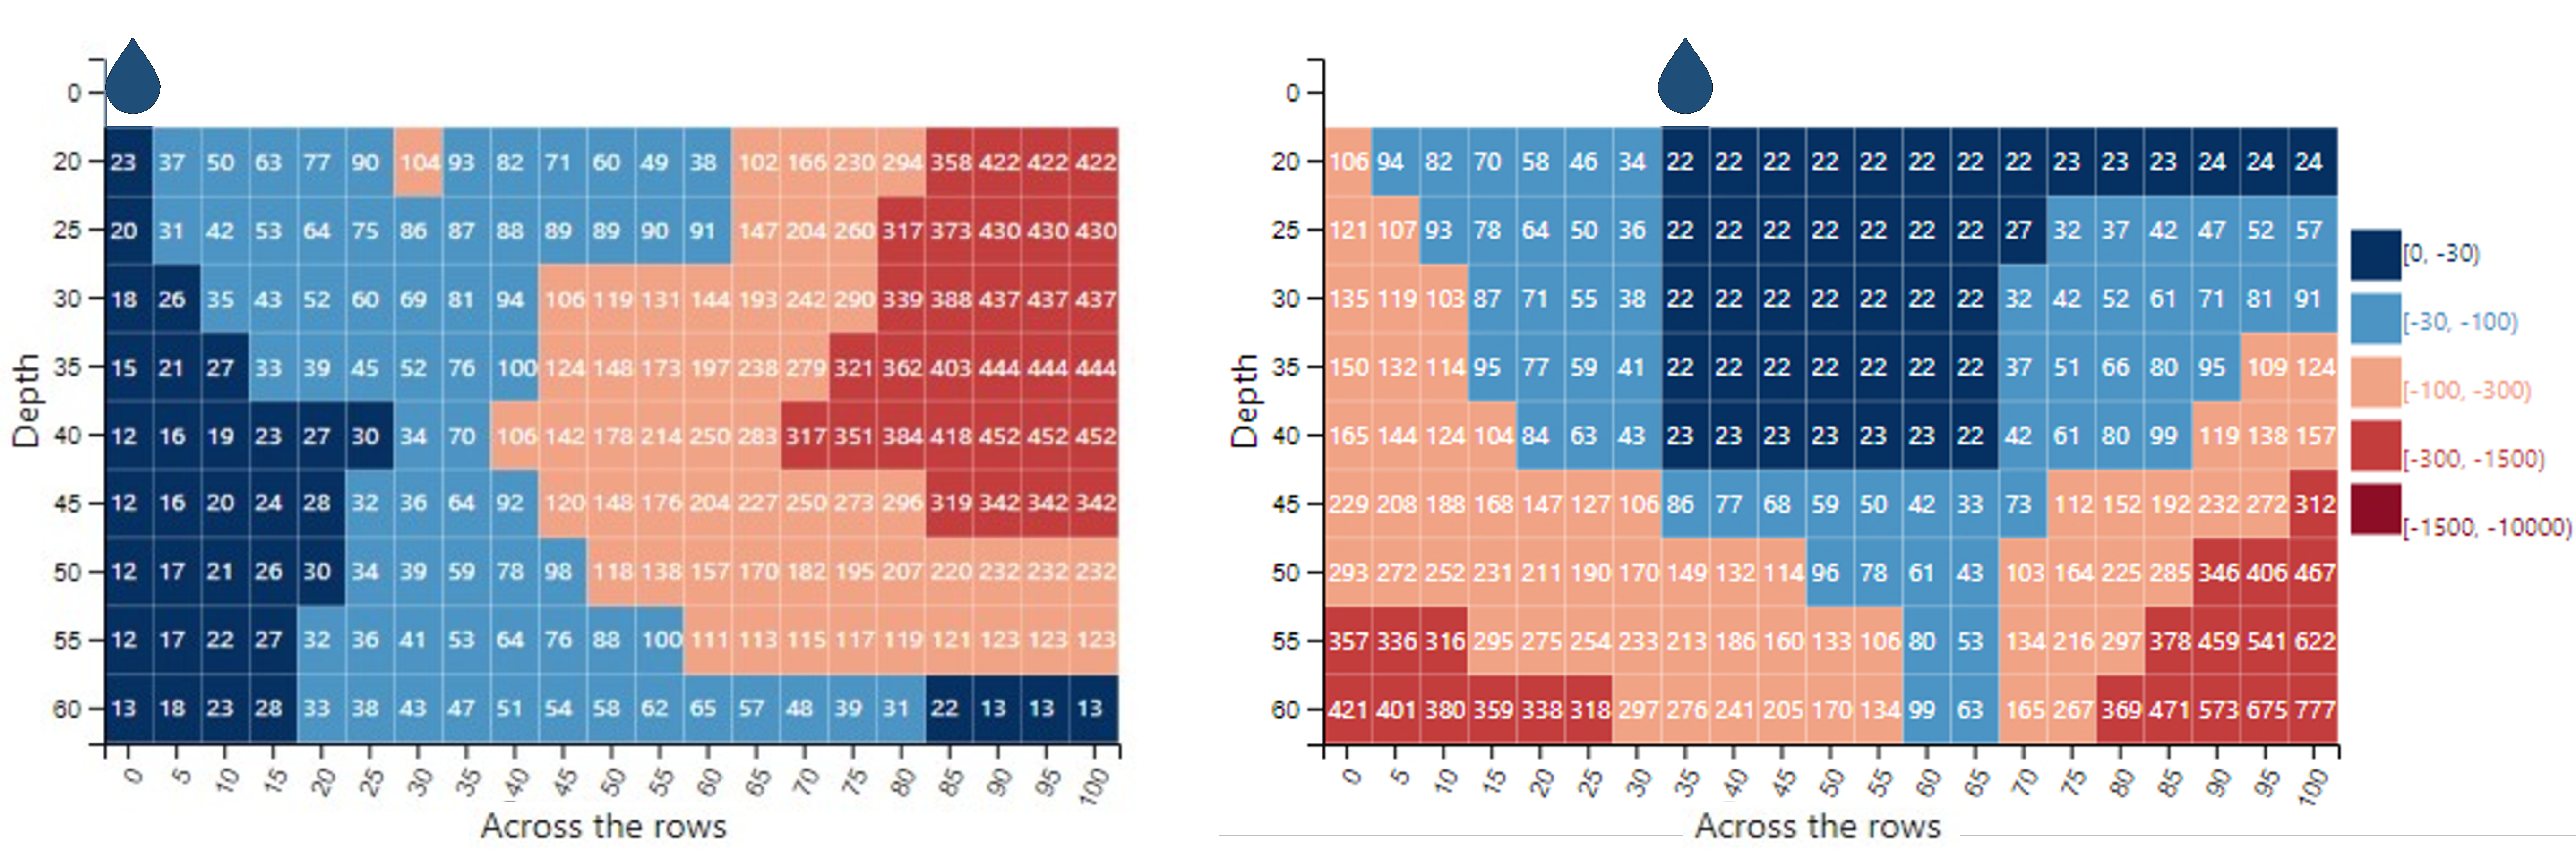
\includegraphics[scale=.13]{chapters/physics-aware/pluto/img/single-double-pipeline.pdf}
\caption{Profile comparison for orchards equipped with single pipeline dripper (left) and double pipeline dripper (right) watering systems. The drop at depth $0$ represents the \textit{Dripper} position and the rightmost legend shows the soil moisture ranges.}
\label{pluto-fig:pipeline-comparison}
\end{figure}

Overall, 2D and 3D profiles are much more accurate; they better capture variations in soil moisture than the baselines (that are traditionally used in commercial settings). \Cref{pluto-fig:pipeline-comparison} highlights the ability to identify different soil behaviors by showing the dynamics of soil moisture in fields with different watering systems. The orchard reported in \Cref{pluto-fig:pipeline-comparison}-left adopts a single-pipeline dripper system where the pipeline is placed along the row. 
The orchard in \Cref{pluto-fig:pipeline-comparison}-right adopts a double-pipeline dripper system were each pipeline is shifted by 20cm on the right/left of the tree row.
As shown by the profile, the compound effect of the raised bed and the shift of the pipeline determines a heavily different soil moisture diffusion.
This effect can only be pointed out using 2D or 3D profiles.

\subsection{Sensor Layout Analysis}
\label{pluto-sec:sensors_disposal_evaluation}
As shown in \Cref{pluto-fig:2Dperformance,fig:3Dperformance}, accuracy varies with the number of sensors. 
Given a regular grid with $n$ sensors, several layouts are possible when $m<n$ sensors are used.  
In particular, while the bilinear feature-unaware function implies some geometric constraints, in the ANN-based feature-aware one all the layouts are feasible.

To compare different layout performances and the system stability with respect to different layouts, we considered the five profiles that achieve the best performances when $m \in [3, 6]$ sensors are used. 
The analysis is carried out in an orchard watered through a single-pipeline dripper system monitored through a grid of $n=12$ sensors (i.e., 4 columns of 3 sensors). 
\Cref{pluto-fig:2D_sensors_importance}
shows the percentage of times the grid sensor appears in one of the top-performing layouts. 
Noticeably, the layouts with highest performance include the sensors that convey more information on soil moisture.
The sensors that turn out to be more relevant are:
\begin{itemize}
    \item the sensor just under the dripper $(0cm, -20cm)$ since it is the most affected by the effects of the dripper;
    \item the sensor near the surface farthest from the dripper $(90cm, -20cm)$ since it records the state of the unwatered volume and is strongly influenced by atmospheric phenomena (e.g., sun, rain, and wind); 
    \item one sensor at mid-depth $(^*, -40cm)$ since it captures the soil behavior when not directly affected by watering and atmospheric phenomena.
\end{itemize}
Besides proving the stability and robustness of the system, this analysis provides the rules for defining the sensor layout.
\begin{figure}[t]
\centering
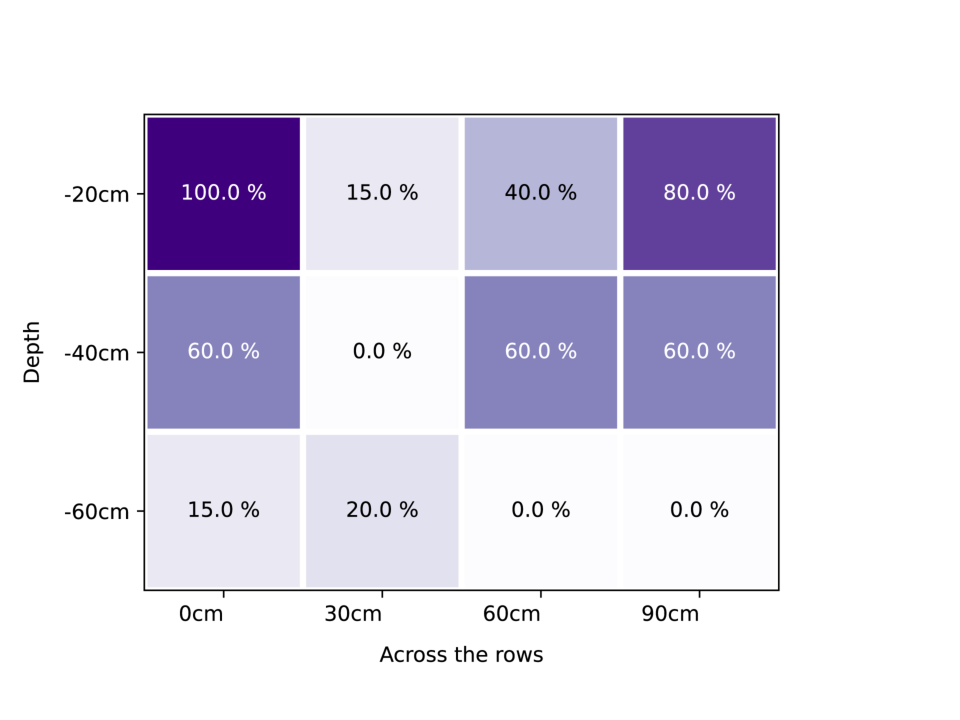
\includegraphics[scale=.6]{chapters/physics-aware/pluto/img/heatmap.pdf}
\caption{Frequency of times each sensor appeared in the best layouts.}
\label{pluto-fig:2D_sensors_importance}
\end{figure}

% \subsection{Effect of PLUTO on Fruit Quantity and Quality}
\subsection{Application of PLUTO in Improving Water Management and Fruit Quality}
\label{pluto-sec:FruitQuality}
We briefly report the results achieved in the Agro.Big.Data.Science project in terms of water saving and fruit quality. Although an in-depth discussion of such results is out of the scope of this chapter, we believe that it is important to demonstrate the ultimate impact of PLUTO; for more details see \cite{quartieri2021effect}. 

We have two irrigation setups during the 2021 campaign (i.e., from May to October 2021) within the same orchard: (i) managed row (irrigation is \textit{automatically} controlled by PLUTO) and (ii) control row (irrigation is \textit{manually} controlled by the farmer). As to (i), given a 2D installation of 12 sensor, the moisture profile was exploited in the water-saving strategy: irrigation was activated when the soil water content got down below the field capacity (-0.003MPa) and returned the same amount of water lost to evapotranspiration the day before (as measured by a PAN evaporimeter \cite{quartieri2021effect}).

As to water saving, the managed row saved $44\%$ of water during the whole campaign. We achieved the maximum saving in June and September when, for the farmer, it is more difficult to accurately estimate the actual soil moisture level and the water requirement.

As to fruit quality, the productivity of vines was unaffected by the irrigation management and ranged from 32 to 39 kg/vine (35-44 t/ha). Fruits from the control row appeared greener with a hue angle of 105 vs a hue angle of 102 for fruits from the managed row. Such fruits also showed a higher soluble solid concentration at harvest: 15.3 brix vs 12.7 brix for the control row. The gap has been maintained after 2 months of storage (and 1 day of shelf life); in particular, the soluble solid concentration was 17.4 brix for the managed rows vs 16.1 brix for the control row.


\section{Conclusions and Future Work}
\label{pluto-sec:conclusions}
We presented PLUTO, an original approach to compute 2D/3D moisture profiles with granularity in the order of magnitude of a few square/cubic centimeters. 
PLUTO relies on a grid of soil moisture sensors and it largely outperforms previous approaches based on a single or a column of sensors. 
To create a  cost-effective operative solution, we have shown that three sensors, properly placed in the soil, are sufficient %to create an effective profile.
to effectively obtain the profiled soil moisture.

We are currently turning our monitoring system into a forecasting one.
We are testing ANNs to create a solution that initially (i.e., before the deployment of the sensors) learns from a soil simulator and then improves its accuracy by exploiting real sensor samples collected during operations. 
The overall goal is to create a prescriptive analytics system that automatically activates the watering system based on a soil moisture forecast module fed with the weather forecast.
